% Options for packages loaded elsewhere
\PassOptionsToPackage{unicode}{hyperref}
\PassOptionsToPackage{hyphens}{url}
%
\documentclass[
  11pt]{article}
\usepackage{amsmath,amssymb}
\usepackage{setspace}
\usepackage{iftex}
\ifPDFTeX
  \usepackage[T1]{fontenc}
  \usepackage[utf8]{inputenc}
  \usepackage{textcomp} % provide euro and other symbols
\else % if luatex or xetex
  \usepackage{unicode-math} % this also loads fontspec
  \defaultfontfeatures{Scale=MatchLowercase}
  \defaultfontfeatures[\rmfamily]{Ligatures=TeX,Scale=1}
\fi
\usepackage{lmodern}
\ifPDFTeX\else
  % xetex/luatex font selection
\fi
% Use upquote if available, for straight quotes in verbatim environments
\IfFileExists{upquote.sty}{\usepackage{upquote}}{}
\IfFileExists{microtype.sty}{% use microtype if available
  \usepackage[]{microtype}
  \UseMicrotypeSet[protrusion]{basicmath} % disable protrusion for tt fonts
}{}
\makeatletter
\@ifundefined{KOMAClassName}{% if non-KOMA class
  \IfFileExists{parskip.sty}{%
    \usepackage{parskip}
  }{% else
    \setlength{\parindent}{0pt}
    \setlength{\parskip}{6pt plus 2pt minus 1pt}}
}{% if KOMA class
  \KOMAoptions{parskip=half}}
\makeatother
\usepackage{xcolor}
\usepackage[margin=22mm]{geometry}
\usepackage{color}
\usepackage{fancyvrb}
\newcommand{\VerbBar}{|}
\newcommand{\VERB}{\Verb[commandchars=\\\{\}]}
\DefineVerbatimEnvironment{Highlighting}{Verbatim}{commandchars=\\\{\}}
% Add ',fontsize=\small' for more characters per line
\newenvironment{Shaded}{}{}
\newcommand{\AlertTok}[1]{\textcolor[rgb]{1.00,0.00,0.00}{\textbf{#1}}}
\newcommand{\AnnotationTok}[1]{\textcolor[rgb]{0.38,0.63,0.69}{\textbf{\textit{#1}}}}
\newcommand{\AttributeTok}[1]{\textcolor[rgb]{0.49,0.56,0.16}{#1}}
\newcommand{\BaseNTok}[1]{\textcolor[rgb]{0.25,0.63,0.44}{#1}}
\newcommand{\BuiltInTok}[1]{\textcolor[rgb]{0.00,0.50,0.00}{#1}}
\newcommand{\CharTok}[1]{\textcolor[rgb]{0.25,0.44,0.63}{#1}}
\newcommand{\CommentTok}[1]{\textcolor[rgb]{0.38,0.63,0.69}{\textit{#1}}}
\newcommand{\CommentVarTok}[1]{\textcolor[rgb]{0.38,0.63,0.69}{\textbf{\textit{#1}}}}
\newcommand{\ConstantTok}[1]{\textcolor[rgb]{0.53,0.00,0.00}{#1}}
\newcommand{\ControlFlowTok}[1]{\textcolor[rgb]{0.00,0.44,0.13}{\textbf{#1}}}
\newcommand{\DataTypeTok}[1]{\textcolor[rgb]{0.56,0.13,0.00}{#1}}
\newcommand{\DecValTok}[1]{\textcolor[rgb]{0.25,0.63,0.44}{#1}}
\newcommand{\DocumentationTok}[1]{\textcolor[rgb]{0.73,0.13,0.13}{\textit{#1}}}
\newcommand{\ErrorTok}[1]{\textcolor[rgb]{1.00,0.00,0.00}{\textbf{#1}}}
\newcommand{\ExtensionTok}[1]{#1}
\newcommand{\FloatTok}[1]{\textcolor[rgb]{0.25,0.63,0.44}{#1}}
\newcommand{\FunctionTok}[1]{\textcolor[rgb]{0.02,0.16,0.49}{#1}}
\newcommand{\ImportTok}[1]{\textcolor[rgb]{0.00,0.50,0.00}{\textbf{#1}}}
\newcommand{\InformationTok}[1]{\textcolor[rgb]{0.38,0.63,0.69}{\textbf{\textit{#1}}}}
\newcommand{\KeywordTok}[1]{\textcolor[rgb]{0.00,0.44,0.13}{\textbf{#1}}}
\newcommand{\NormalTok}[1]{#1}
\newcommand{\OperatorTok}[1]{\textcolor[rgb]{0.40,0.40,0.40}{#1}}
\newcommand{\OtherTok}[1]{\textcolor[rgb]{0.00,0.44,0.13}{#1}}
\newcommand{\PreprocessorTok}[1]{\textcolor[rgb]{0.74,0.48,0.00}{#1}}
\newcommand{\RegionMarkerTok}[1]{#1}
\newcommand{\SpecialCharTok}[1]{\textcolor[rgb]{0.25,0.44,0.63}{#1}}
\newcommand{\SpecialStringTok}[1]{\textcolor[rgb]{0.73,0.40,0.53}{#1}}
\newcommand{\StringTok}[1]{\textcolor[rgb]{0.25,0.44,0.63}{#1}}
\newcommand{\VariableTok}[1]{\textcolor[rgb]{0.10,0.09,0.49}{#1}}
\newcommand{\VerbatimStringTok}[1]{\textcolor[rgb]{0.25,0.44,0.63}{#1}}
\newcommand{\WarningTok}[1]{\textcolor[rgb]{0.38,0.63,0.69}{\textbf{\textit{#1}}}}
\usepackage{longtable,booktabs,array}
\usepackage{calc} % for calculating minipage widths
% Correct order of tables after \paragraph or \subparagraph
\usepackage{etoolbox}
\makeatletter
\patchcmd\longtable{\par}{\if@noskipsec\mbox{}\fi\par}{}{}
\makeatother
% Allow footnotes in longtable head/foot
\IfFileExists{footnotehyper.sty}{\usepackage{footnotehyper}}{\usepackage{footnote}}
\makesavenoteenv{longtable}
\usepackage{graphicx}
\makeatletter
\def\maxwidth{\ifdim\Gin@nat@width>\linewidth\linewidth\else\Gin@nat@width\fi}
\def\maxheight{\ifdim\Gin@nat@height>\textheight\textheight\else\Gin@nat@height\fi}
\makeatother
% Scale images if necessary, so that they will not overflow the page
% margins by default, and it is still possible to overwrite the defaults
% using explicit options in \includegraphics[width, height, ...]{}
\setkeys{Gin}{width=\maxwidth,height=\maxheight,keepaspectratio}
% Set default figure placement to htbp
\makeatletter
\def\fps@figure{htbp}
\makeatother
\setlength{\emergencystretch}{3em} % prevent overfull lines
\providecommand{\tightlist}{%
  \setlength{\itemsep}{0pt}\setlength{\parskip}{0pt}}
\setcounter{secnumdepth}{-\maxdimen} % remove section numbering
\ifLuaTeX
\usepackage[bidi=basic]{babel}
\else
\usepackage[bidi=default]{babel}
\fi
\babelprovide[main,import]{british}
% get rid of language-specific shorthands (see #6817):
\let\LanguageShortHands\languageshorthands
\def\languageshorthands#1{}
% Preamble for JLC submission (article class, pdfLaTeX + UTF-8)
\usepackage[utf8]{inputenc}
\usepackage[T1]{fontenc}
\usepackage{textcomp}
\usepackage{lmodern}
\usepackage[margin=22mm]{geometry}
\usepackage{microtype}
\usepackage{graphicx}
\setkeys{Gin}{width=\linewidth,height=0.85\textheight,keepaspectratio}
\usepackage{booktabs}
\usepackage{longtable}
\usepackage{array}
\usepackage{hyperref}
\hypersetup{colorlinks=true, linkcolor=blue, citecolor=blue, urlcolor=blue}
\usepackage{enumitem}
\setlist{nosep}
\usepackage{amsmath,amssymb}
\usepackage{xcolor}
\usepackage{fvextra}
\DefineVerbatimEnvironment{Highlighting}{Verbatim}{breaklines=true,breakanywhere=true,fontsize=\small,commandchars=\\\{\}}
\usepackage{newunicodechar}
\newunicodechar{§}{\S}
\newunicodechar{₁}{\ensuremath{_1}}
\newunicodechar{₂}{\ensuremath{_2}}
\newunicodechar{ₙ}{\ensuremath{_n}}
\providecommand{\tightlist}{\setlength{\itemsep}{0pt}\setlength{\parskip}{0pt}}
% Headings carry manual numbers (e.g. "9. Conclusion"); disable LaTeX's own.
\setcounter{secnumdepth}{-\maxdimen}
\ifLuaTeX
  \usepackage{selnolig}  % disable illegal ligatures
\fi
\IfFileExists{bookmark.sty}{\usepackage{bookmark}}{\usepackage{hyperref}}
\IfFileExists{xurl.sty}{\usepackage{xurl}}{} % add URL line breaks if available
\urlstyle{same}
\hypersetup{
  pdftitle={Proof Graphs and Algorithm Capsules: A Corpus Study of Diagonalization Proofs from Cantor to Gödel to Goodstein},
  pdfauthor={Gary Welz},
  pdflang={en-GB},
  pdfkeywords={mathematical knowledge representation, proof graphs,
axiomatic systems, LLM-generated diagrams, Mermaid, process
visualization, graph-theoretic representation, Programming Framework},
  hidelinks,
  pdfcreator={LaTeX via pandoc}}

\title{Proof Graphs and Algorithm Capsules: A Corpus Study of
Diagonalization Proofs from Cantor to Gödel to Goodstein}
\author{Gary Welz \\[0.6em]{\normalsize Researcher, New Media Lab, CUNY Graduate Center} \\[0.35em]{\normalsize Email: \texttt{gwelz@gc.cuny.edu}} \\[0.35em]{\normalsize ORCID: \url{https://orcid.org/0009-0005-7806-0892}}}
\date{}

\begin{document}
\maketitle
\begin{abstract}
Mathematics encompasses three fundamentally distinct object types ---
algorithms, axiomatic systems, and proofs. These are conventionally
treated as categorically separate in mathematical practice, education,
and knowledge representation. We demonstrate that all three can be
expressed as labeled directed graphs using Mermaid Markdown. This
unified representation reveals structural properties that conventional
prose and static diagrams obscure. The central empirical finding is the
regularity of \textbf{algorithm capsules} --- embedded procedural
substructures within proofs --- across mathematically distant domains.
Analysis of the Mathematics Database corpus identifies a
\textbf{diagonalization family} spanning three entries: Cantor diagonal
proofs, the Gödel First Incompleteness proof graph, and the
Kirby--Paris/Goodstein independence result. In each case the algorithm
capsule is not incidental to the argument but is its structural core.
This family resemblance is visible and measurable in the graph
representation. It is not accessible from prose alone. The
representation is implemented as three graph types. Algorithmic
flowcharts capture procedural structure. Axiomatic dependency graphs
represent logical dependency among axioms, definitions, and theorems.
Proof graphs --- a hybrid form introduced here --- encode justification
structure using a domain-specific eight-role node vocabulary: source,
assumption, construction, assertion, inference, algorithm capsule,
contradiction, and conclusion. Together the three graph types constitute
the Mathematics Database, a publicly accessible machine-readable corpus
spanning classical geometry, number theory, algebra, set theory,
mathematical logic, and theoretical computer science. The methodology is
a domain-specific application and extension of the Programming
Framework, a general method for LLM-assisted process visualization. The
mathematics case demonstrates that the framework\textquotesingle s core
claim extends from procedural processes to logical and justificatory
structures: that formal structure is recoverable from natural language
descriptions of complex systems, and is meaningful, measurable, and
comparable once recovered.
\end{abstract}

\setstretch{1.15}
\hypertarget{1-introduction}{%
\subsection{1. Introduction}\label{1-introduction}}

\hypertarget{11-the-representation-problem-in-mathematical-proofs}{%
\subsubsection{1.1 The Representation Problem in Mathematical
Proofs}\label{11-the-representation-problem-in-mathematical-proofs}}

Mathematical proofs are structured arguments in which assumptions,
constructions, inferences, and conclusions carry distinct logical roles.
Yet proofs are almost always published and taught in prose --- linear
text that conceals the dependency structure of the argument, obscures
where procedural constructions sit within inferential steps, and offers
no common format for comparing proofs across domains or methods.

This representational gap has consequences. A logician reading
Gödel\textquotesingle s incompleteness proof and a set theorist reading
Cantor\textquotesingle s diagonal argument may each recognize that a
diagonal construction lies at the core of the argument, but comparing
the structural role of those constructions --- or measuring how each
proof allocates complexity between procedure and inference --- requires
placing both arguments in a common representational space. That space
does not exist in standard mathematical practice. Knowledge
representation systems typically address axiomatic dependency charts or
formal verification certificates, not the internal architecture of
informal proof arguments as inspectable, comparable structures.

Algorithms and axiomatic systems --- the other object types
mathematicians work with routinely --- suffer parallel representational
fragmentation: procedures appear as pseudocode or flowcharts, theories
as numbered axiom lists. This paper concentrates on proofs. The question
is whether proof structure can be made explicit, measurable, and
comparable --- and whether doing so reveals regularities invisible in
prose.

\hypertarget{12-the-proposed-approach}{%
\subsubsection{1.2 The Proposed
Approach}\label{12-the-proposed-approach}}

This paper concentrates on \textbf{proof graphs} --- labeled directed
graphs that encode the justification structure of mathematical arguments
--- though the same pipeline also produces algorithmic flowcharts and
axiomatic dependency graphs for comparative context (§3.1--§3.2, §6.2).
The central empirical thread is a corpus study of eight proof graphs,
with particular attention to three landmark diagonalization arguments:
Cantor\textquotesingle s diagonal proofs, Gödel\textquotesingle s First
Incompleteness Theorem, and the Kirby--Paris/Goodstein independence
result. Represented as proof graphs, these three proofs --- usually
treated as belonging to set theory, mathematical logic, and
combinatorics respectively --- share a common structural signature: in
each case an \textbf{algorithm capsule} (an embedded procedural
substructure) is not incidental to the argument but is its structural
core. We term this group the \textbf{diagonalization family}; the
finding is developed with exact corpus figures in §6.

Proof graphs expose the roles played by different proof steps, the
presence of algorithm capsules, and the structural differences between
proofs of the same theorem by different methods. Algorithmic flowcharts
and axiomatic dependency graphs, generated by the same methodology,
provide the comparative baseline against which proof-graph complexity
can be measured.

A skeptical reader might ask whether the graph representation merely
redescribes what a careful reader of the prose already knows, rather
than revealing anything genuinely new. The answer is that making
structure explicit is itself a form of discovery --- specifically when
the structure was previously inaccessible to measurement and comparison.
Comparing the construction in Euclid\textquotesingle s infinitude
argument to the diagonal constructions in Cantor, Gödel, and Goodstein
requires a common representational space. The graph provides that space.
It is what makes the diagonalization family observation a finding rather
than a redescription. The situation is analogous to phylogenetic trees
in biology: evolutionary relationships were always present, but the tree
representation made them comparable, measurable, and falsifiable in a
way that prose natural history did not.

The mechanism for generating these graphs is the Programming Framework:
a methodology for transforming natural language descriptions of
processes into structured Mermaid Markdown diagrams using large language
models (LLMs), with human-in-the-loop validation and versioned JSON
storage {[}1{]}.

\hypertarget{13-contributions}{%
\subsubsection{1.3 Contributions}\label{13-contributions}}

This paper contributes:

\textbf{Conceptual:} A proof-graph formalism with an eight-role node
vocabulary (source, assumption, construction, assertion, inference,
algorithm capsule, contradiction, conclusion) and the algorithm capsule
as a representational device for embedded procedural substructures
within proofs.

\textbf{Empirical:} A corpus study of eight proof graphs, with the
identification of the diagonalization family spanning Cantor, Gödel, and
Goodstein --- three proofs whose shared topological signature is visible
and measurable in the graph representation but not recoverable from
prose alone. The Mathematics Database provides the open,
machine-readable infrastructure for this corpus.

\textbf{Methodological:} A human-in-the-loop pipeline for generating
proof graphs from natural language descriptions using LLMs, as a
domain-specific extension of the Programming Framework {[}1{]}.

\textbf{Theoretical:} The claim that proof graphs regularly contain
algorithm capsules, making explicit a structural relationship between
proof and computation that is implicit in mathematical practice but
rarely formalized at the diagram level --- and that this relationship
intensifies in diagonalization arguments across mathematically distant
domains.

\begin{center}\rule{0.5\linewidth}{0.5pt}\end{center}

\hypertarget{2-related-work}{%
\subsection{2. Related Work}\label{2-related-work}}

\hypertarget{21-graph-based-proof-representation}{%
\subsubsection{2.1 Graph-Based Proof
Representation}\label{21-graph-based-proof-representation}}

Graph-theoretic representations of proofs have been explored in proof
complexity theory {[}9{]}, where proof graphs (also called proof DAGs)
are used to measure the size and depth of proofs in formal systems. DAG
stands for directed acyclic graph: edges flow in one direction, and no
step can depend, even indirectly, on itself. DAG-like proofs have been
studied as a generalization of tree-like proofs {[}9{]}.

The proof graphs in this paper are DAGs at the proof level. Several
corpus entries contain algorithm capsule nodes whose internal structure
is cyclic --- the diagonal enumeration in the Rationals Are Countable
proof, for example, contains an explicit loop. The algorithm capsule
node type makes this two-level structure visible: cycles are
encapsulated within capsule nodes rather than appearing at the proof
graph\textquotesingle s top level.

The present work differs from proof complexity in that it is concerned
with the semantic roles of nodes in proofs --- what each step does
(assumption, construction, inference, and so on) --- rather than with
formal complexity bounds. Argument mapping {[}10{]} is a closer
conceptual relative: the proof graph vocabulary in §3.3 can be
understood as a domain-specific formalization of argument mapping
applied to mathematical justification.

Formal proof assistants --- Lean {[}3{]}, Coq {[}5{]}, Isabelle {[}6{]}
--- represent mathematics for machine verification rather than
structural inspection. Section 4.1 contrasts Lean-style proof flow with
the informal proof graphs used here; the two approaches are
complementary, not competing.

\hypertarget{22-llm-diagram-generation}{%
\subsubsection{2.2 LLM Diagram
Generation}\label{22-llm-diagram-generation}}

Large language models have demonstrated capacity for mathematical
reasoning {[}11, 12{]}, and recent work has explored LLM-assisted
formalization of mathematics {[}13{]}. The present work uses LLMs
differently: not to reason about mathematics or verify proofs, but to
generate structured diagrammatic representations from natural language
descriptions, as one step in a human-in-the-loop pipeline. This paper
makes no claims about LLM mathematical reasoning ability, only about LLM
utility as a diagram generation tool under human supervision.

\hypertarget{23-programming-framework-and-generation-pipeline}{%
\subsubsection{2.3 Programming Framework and Generation
Pipeline}\label{23-programming-framework-and-generation-pipeline}}

The Programming Framework {[}1{]} is a general methodology for
transforming textual process descriptions into structured Mermaid
Markdown diagrams {[}14{]} using LLMs, with human-in-the-loop validation
and versioned JSON storage. The present paper extends it to proof graphs
by introducing the eight-role node vocabulary and algorithm capsule
concept described in §3.3.

All proof graphs in the corpus were generated using the following
pipeline:

\textbf{Step 1 --- Source selection.} A proof is selected and a natural
language description is prepared from standard reference sources ---
typically textbook or encyclopaedia prose.

\textbf{Step 2 --- LLM prompting.} The description is submitted to a
large language model with a structured prompt specifying the proof-graph
node vocabulary, color scheme, and Mermaid syntax requirements.

\textbf{Step 3 --- Human review.} The generated diagram is rendered and
reviewed for logical dependency accuracy, node coverage, role
assignment, and Mermaid validity.

\textbf{Step 4 --- Metadata construction.} A JSON metadata record is
constructed per the schema in §5.1; structural metrics are counted from
the rendered diagram.

\textbf{Step 5 --- Versioned storage.} The completed entry is committed
to the Google Cloud Storage repository and made publicly accessible via
the interactive viewer in §5.4.

The human review step is the primary quality control mechanism. It does
not constitute formal expert validation --- that limitation is noted in
§7 --- but it ensures that each entry has been inspected for logical
accuracy by an author with familiarity with the relevant mathematical
content.

\begin{center}\rule{0.5\linewidth}{0.5pt}\end{center}

\hypertarget{3-the-three-graph-types}{%
\subsection{3. The Three Graph Types}\label{3-the-three-graph-types}}

\hypertarget{31-algorithmic-flowcharts}{%
\subsubsection{3.1 Algorithmic
Flowcharts}\label{31-algorithmic-flowcharts}}

An algorithmic flowchart in the Mathematics Database is a standard
directed graph where:

\begin{itemize}
\tightlist
\item
  \textbf{Nodes} represent computational steps, decisions, or states
\item
  \textbf{Edges} represent sequential or conditional flow
\item
  \textbf{Node colors} follow the Programming
  Framework\textquotesingle s five-category system: Red (inputs), Yellow
  (data structures/algorithms), Green (operations), Blue (intermediate
  states/decisions), Violet (outputs/results)
\item
  \textbf{AND gates} represent steps that require multiple prior
  conditions to be satisfied before proceeding
\item
  \textbf{OR gates} (decision nodes) represent conditional branches
  where one of several paths is taken
\item
  \textbf{Loops} (back-edges) represent iterative or recursive structure
\end{itemize}

\textbf{Structural metrics captured:} node count, edge count,
conditional count, AND gate count, OR gate count, loop count, graph
type.

\textbf{Examples in the database:}

\begin{itemize}
\tightlist
\item
  Sieve of Eratosthenes --- high loop depth, iterative primality marking
\item
  Merge Sort --- recursive structure, divide-and-conquer branching
\item
  Dijkstra\textquotesingle s Algorithm --- priority queue management,
  relaxation loop
\item
  Euclidean Algorithm --- minimal loop, elegant termination condition
\item
  Binary Search --- logarithmic branching structure
\end{itemize}

Figure 1 illustrates the Euclidean Algorithm as an algorithmic flowchart
using this color vocabulary. The algorithm is a clean example of
iterative structure: a single decision node, a back-edge forming the
loop, and a minimal path to termination. The color legend appears with
the diagram.

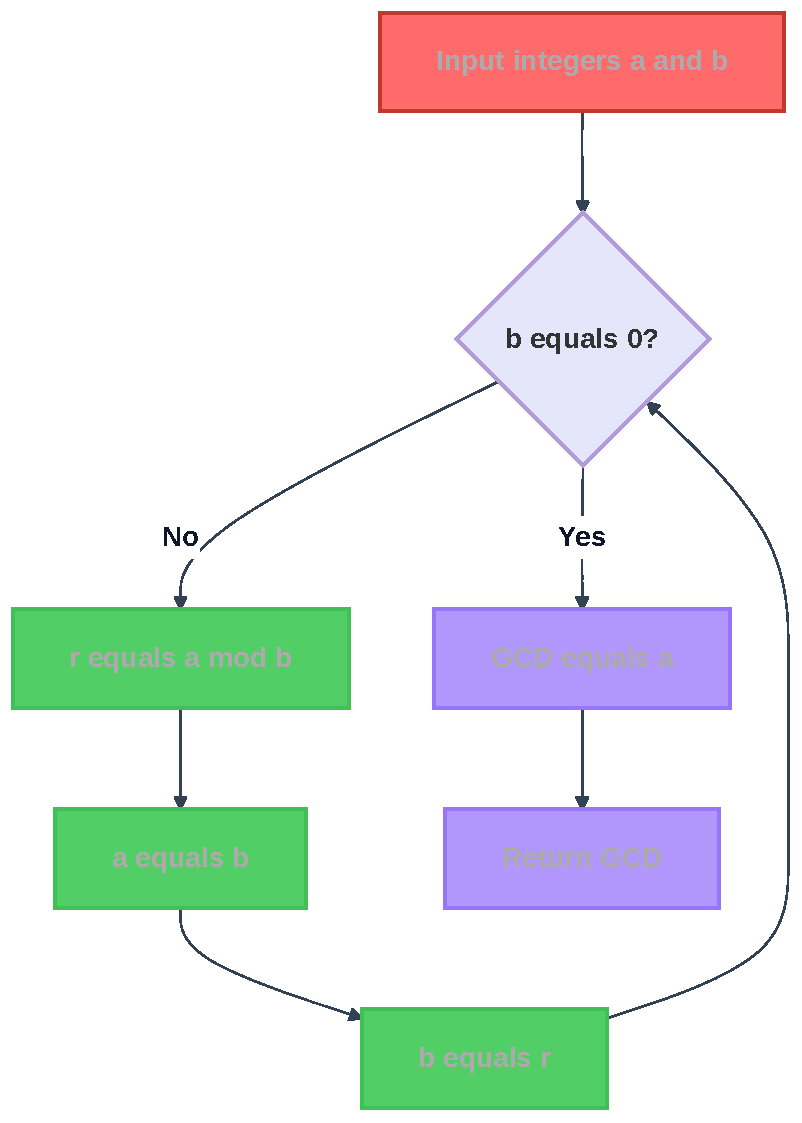
\includegraphics{figures/fig1.pdf}

\emph{Figure 1: Euclidean Algorithm --- algorithmic flowchart. GLMP
6-color scheme (exact hex values from the Mathematics Database table):
Red = input, Lavender = decision, Green = operation, Violet = output.}

Algorithmic flowcharts are the most direct application of the
Programming Framework\textquotesingle s base methodology and require no
extension to the standard vocabulary.

\hypertarget{32-axiomatic-dependency-graphs}{%
\subsubsection{3.2 Axiomatic Dependency
Graphs}\label{32-axiomatic-dependency-graphs}}

An axiomatic dependency graph represents the logical architecture of a
mathematical system as a directed acyclic graph (DAG) --- the same
structure defined in §2.1, where edges flow in one direction and no
theorem can depend, even indirectly, on itself. In the axiomatic
context, acyclicity is not merely a formal property but a logical
requirement: if theorem B depends on theorem A, then A cannot
simultaneously depend on B, or the entire deductive structure would be
circular and the system would prove nothing.

The nodes and edges of an axiomatic dependency graph are:

\begin{itemize}
\tightlist
\item
  \textbf{Nodes} represent mathematical objects: Axiom, Definition,
  Lemma, Theorem, Corollary, Postulate, Primitive (undefined term)
\item
  \textbf{Edges} represent logical dependency: an edge from A to B means
  B depends on, uses, or requires A
\item
  \textbf{Node colors} encode object type: a domain-specific extension
  of the Programming Framework\textquotesingle s color system applied to
  logical roles rather than process stages
\item
  \textbf{Depth from axioms} measures how many inference steps separate
  a theorem from first principles
\end{itemize}

\textbf{Structural metrics captured:} node count, edge count, depth
distribution, axiom-to-theorem ratio, number of distinct proof paths to
key results.

\textbf{Examples in the database:} Euclid\textquotesingle s Elements,
Peano Arithmetic, ZFC Set Theory, and standard algebraic theories ---
194 entries in total, listed in the live database (§5.4). This paper
does not survey them entry by entry; they supply comparative context in
§6.2.

Figure 2 gives an illustrative dependency slice of Book I of
Euclid\textquotesingle s Elements --- postulates, common notions, and
early propositions --- with coloring by object type. Node labels are
abbreviated after Heath\textquotesingle s translation.

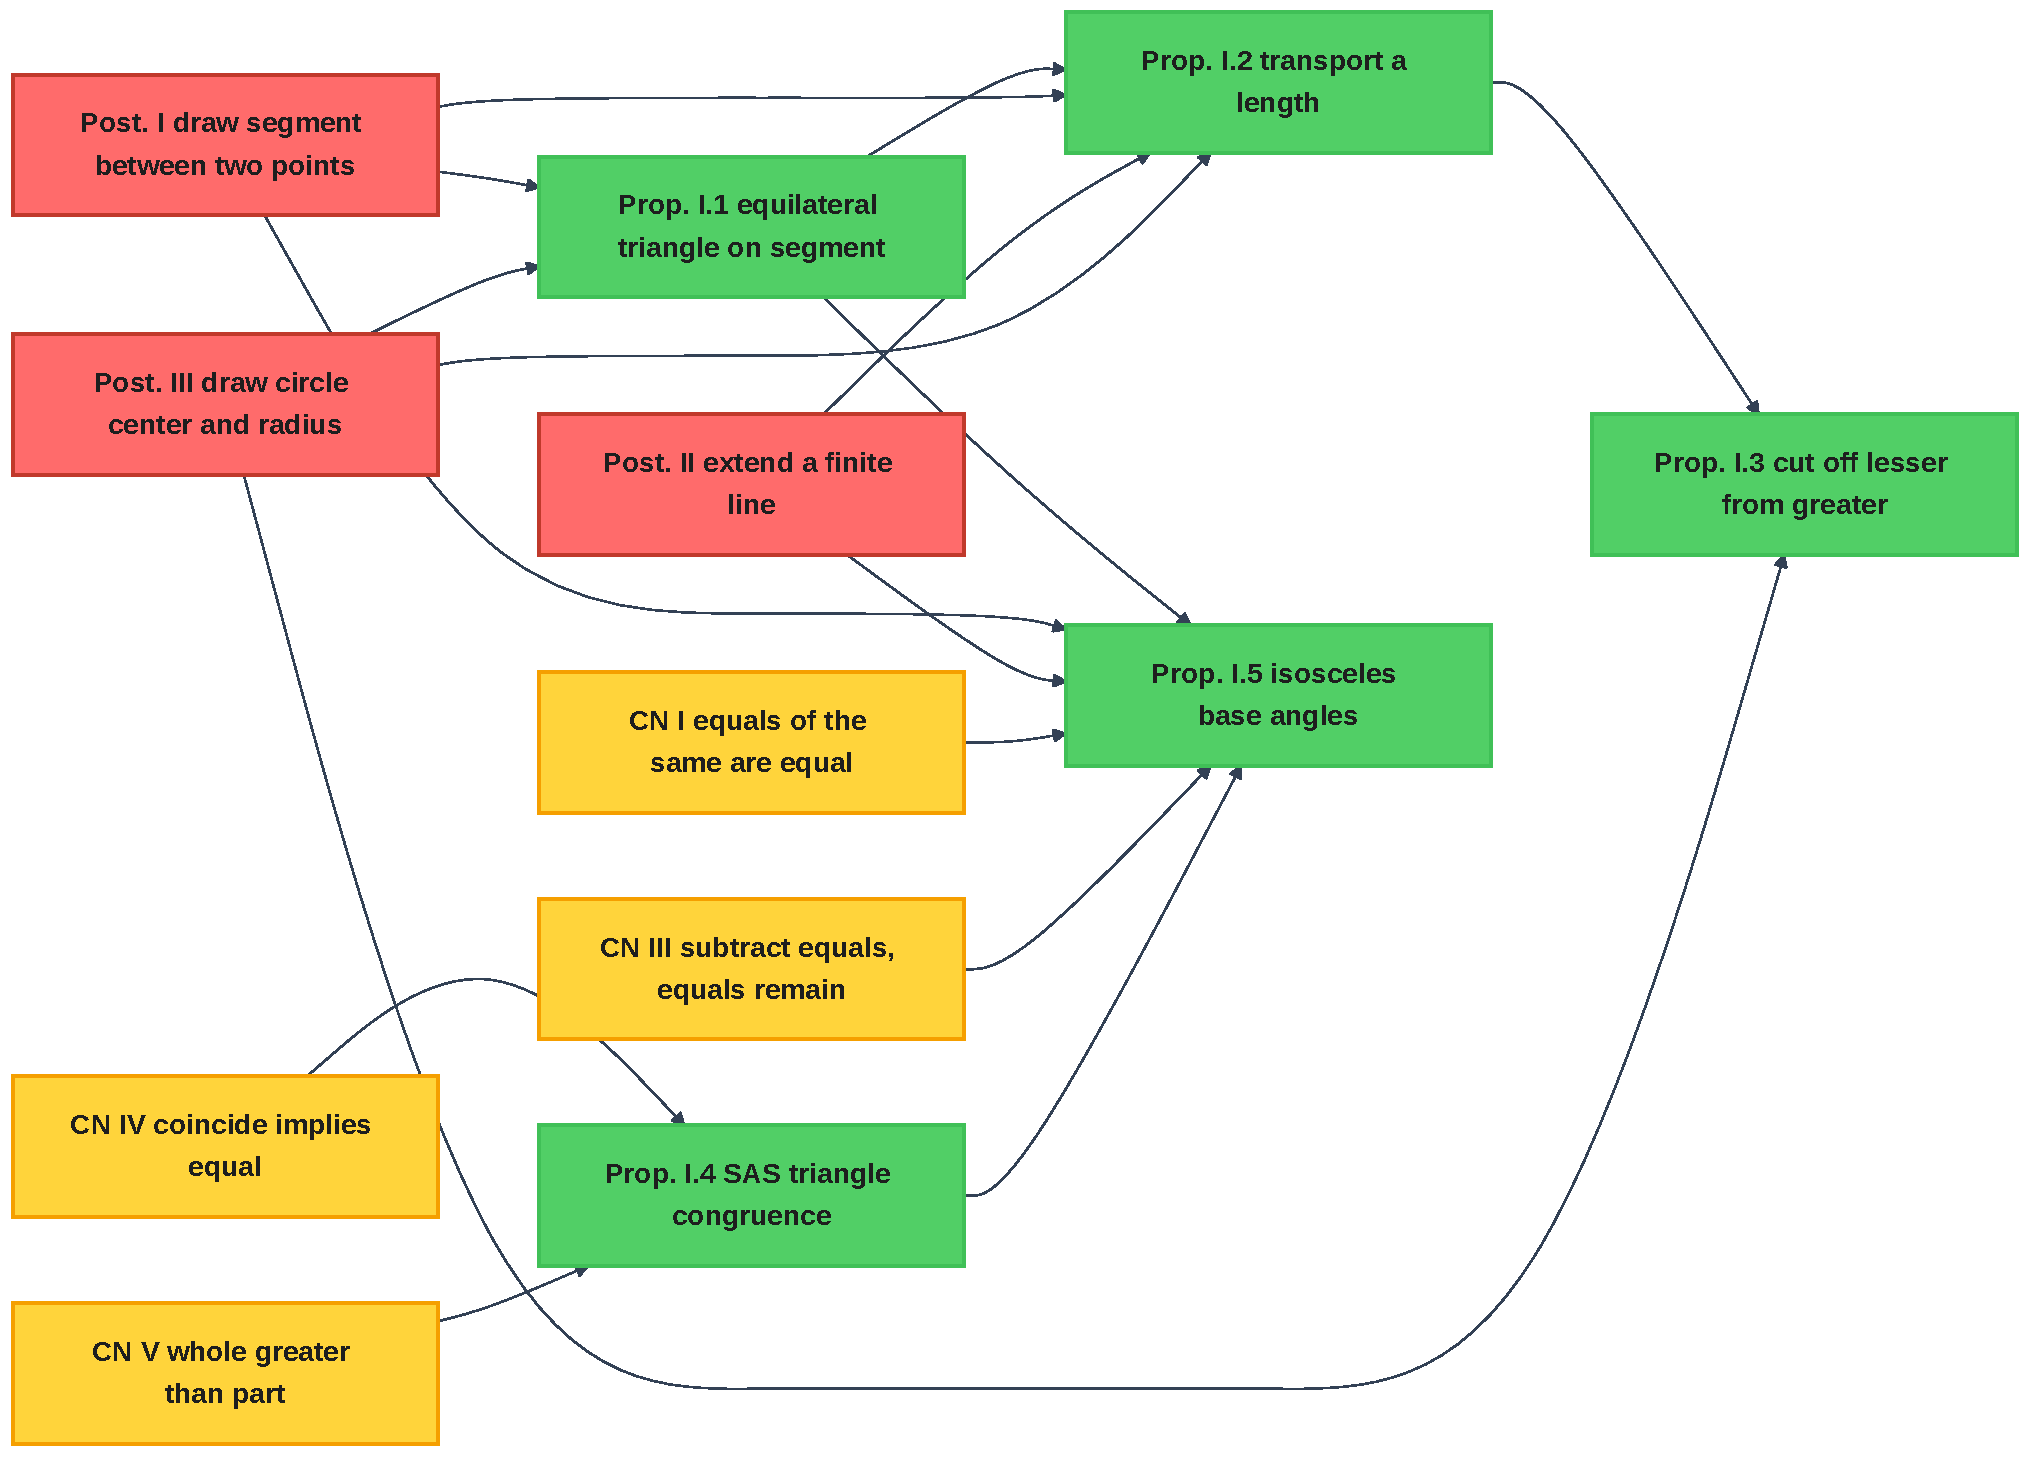
\includegraphics{figures/fig2.pdf}

\emph{Figure 2: Euclid\textquotesingle s Elements Book I --- axiomatic
dependency graph (illustrative; abbreviated node labels after Heath).
Database palette: Red = Postulates, Yellow = Common Notions, Green =
Propositions.}

Axiomatic dependency graphs require a domain-specific node vocabulary
not present in the base Programming Framework, making them a natural
extension case. The acyclicity of these graphs is not imposed as a
technical constraint but follows from the logical requirement that
deductive systems be non-circular.

\hypertarget{33-proof-graphs}{%
\subsubsection{3.3 Proof Graphs}\label{33-proof-graphs}}

Proof graphs are the novel contribution of this paper. A proof graph
represents the justification structure of a mathematical proof as a
directed graph where:

\begin{itemize}
\tightlist
\item
  \textbf{Nodes} carry an eight-role vocabulary encoding the
  proof-theoretic function of each step
\item
  \textbf{Edges} represent logical dependency: an edge from A to B means
  B follows from, depends on, or uses A
\item
  \textbf{Node colors} encode proof role, not process stage --- a
  domain-specific extension of the Programming
  Framework\textquotesingle s color system
\end{itemize}

\textbf{Proof graphs and acyclicity.} At the proof level, proof graphs
are DAGs: logical dependency flows in one direction from premises to
conclusion, and no step can depend, even indirectly, on itself. However,
proof graphs differ from axiomatic dependency graphs in one important
structural respect: they may contain algorithm capsule nodes whose
internal structure is cyclic. The diagonal enumeration in the Rationals
Are Countable proof contains an explicit loop; the anti-diagonal
constructions in the Reals Are Uncountable and Cantor Power Set proofs
encapsulate iterative procedures. The algorithm capsule node type is the
representational device that makes this two-level structure visible and
precise: cycles are encapsulated within capsule nodes rather than
appearing at the proof graph\textquotesingle s top level. This
distinction --- between proof-level acyclicity and capsule-level
iteration --- is one of the structural properties the unified
representation makes explicit that prose cannot.

\textbf{The eight-role proof graph vocabulary:}

\begin{longtable}[]{@{}>{\raggedright\arraybackslash}p{0.16\linewidth}>{\raggedright\arraybackslash}p{0.38\linewidth}>{\raggedright\arraybackslash}p{0.36\linewidth}@{}}
\toprule\noalign{}
Role & GLMP color & Definition \\
\midrule\noalign{}
\endhead
\bottomrule\noalign{}
\endlastfoot
Source & Red (\texttt{\#ff6b6b}) & The theorem, proposition, or claim
being proved \\
Assumption & Yellow (\texttt{\#ffd43b}) & A temporary assumption (e.g.,
for contradiction or induction) \\
Construction & Yellow (\texttt{\#ffd43b}) & An object explicitly
constructed in the proof \\
Assertion & Green (\texttt{\#51cf66}) & A claim that follows from prior
steps \\
Inference & Light blue (\texttt{\#74c0fc}) & A logical inference rule or
proof step \\
Algorithm Capsule & Green (\texttt{\#51cf66}) & An embedded algorithmic
substructure within the proof \\
Contradiction & Red (\texttt{\#ff6b6b}) & A contradiction reached (in
proof by contradiction) \\
Conclusion & Violet (\texttt{\#b197fc}) & The final conclusion
establishing the theorem \\
\end{longtable}

All figures in this paper use the \textbf{exact GLMP 6-color fills} from
the Mathematics Database table viewer: red, yellow, green, light blue,
violet, and lavender (decision diamonds). Node labels are rendered in
dark text (\texttt{\#1e1e1e}) for print/PDF readability on the pastel
fills. Proof roles map onto this palette as shown above.

\textbf{A note on rendering.} The live proof-graph entry pages in the
Mathematics Database render the same eight roles with a dedicated
eight-hue legend --- amber (source), violet (assumption), moss
(construction), steel (assertion), copper (inference), indigo (algorithm
capsule), crimson (contradiction), teal (conclusion) --- assigning each
role its own hue against the pages\textquotesingle{} dark theme. The
figures in this paper instead map the eight roles onto the table
viewer\textquotesingle s six-color palette, for consistency with the
database\textquotesingle s other graph types and for legibility in
print. In both renderings the role semantics are carried by the node
labels; the role vocabulary, not the hue assignment, is normative.

\textbf{On the mutual exclusivity of roles.} The eight roles are
intended to be mutually exclusive: each node in a proof graph carries
exactly one role. In practice, some proof steps are ambiguous --- a step
may function simultaneously as a construction and an assertion, or as an
inference and a conclusion. The decision rule applied in the Mathematics
Database is to assign the role that best captures the
step\textquotesingle s primary proof-theoretic function. A step that
constructs an object and asserts a property of it in the same move is
classified as a Construction if the object\textquotesingle s existence
is what the proof requires, and as an Assertion if the property is what
the proof requires. A step that draws a final inference is classified as
a Conclusion rather than an Inference if it directly establishes the
theorem being proved. These decisions are recorded in the entry metadata
and are available for review. The goal is consistency within the corpus
rather than a claim that the boundaries are always sharp.

\textbf{The algorithm capsule concept.} An algorithm capsule is a node
representing an embedded procedural substructure within a proof --- an
explicit construction or procedure that is carried out within the proof
argument and is distinct in character from the logical inference steps
surrounding it. Algorithm capsules are the most structurally significant
node type in the proof graph vocabulary for two reasons.

First, they mark the boundary between the algorithmic and the
inferential within a single proof. In Euclid\textquotesingle s proof of
the infinitude of primes, the construction of N = p₁p₂...pₙ + 1 is an
algorithm capsule: it is a finite procedure whose output --- a number
not divisible by any listed prime --- is what the
proof\textquotesingle s contradiction depends on. The inferential steps
before and after the capsule are logically dependent on the
capsule\textquotesingle s output but are not themselves algorithmic.
Making this boundary explicit as a node type reveals a structural
relationship between proof and computation that is normally invisible in
prose.

Second, as noted above, algorithm capsules are the location within proof
graphs where cyclic structure --- iterative or recursive procedures ---
appears. The proof graph remains a DAG at its top level; the cycles are
contained within capsule nodes. This encapsulation is not a limitation
of the representation but a feature: it preserves the DAG structure of
the proof\textquotesingle s logical dependency while accurately
representing the computational structure of its embedded procedures.

\textbf{Examples in the database:}

\emph{Euclid Book I Pilot Proofs} (41 nodes, 48 edges, hybrid graph
type) --- the foundational geometric proofs; rich in construction nodes;
one algorithm capsule in I.1 (compass-and-straightedge construction).

\emph{Infinitely Many Primes} (14 nodes, 17 edges, contradiction
structure) --- Euclid\textquotesingle s proof; compact graph with clear
contradiction arc and a central algorithm capsule (construction of N =
p₁p₂...pₙ + 1).

\emph{Pythagorean Theorem Proof Comparison} (33 nodes, 39 edges,
multiple proof families) --- graph representation of multiple distinct
proofs of the same theorem; structural differences between proof
families become visually and metrically comparable.

\emph{Fundamental Theorem of Arithmetic} (27 nodes, 34 edges) --- the
unique prime factorization theorem; graph reveals the two-part structure
(existence and uniqueness) and their distinct dependency chains.

\emph{Cantor Diagonal Proofs} (42 nodes, 50 edges, hybrid family) ---
Cantor\textquotesingle s diagonal argument in multiple variants;
algorithm capsule is the structural core of all variants; graph reveals
the family resemblance across proof variants and the two-level DAG/cycle
structure described above.

\emph{Gödel Completeness Theorem} (15 nodes, 15 edges) --- proof graph
pilot; dependency structure of the completeness argument; one algorithm
capsule.

\emph{Gödel First Incompleteness Theorem} (14 nodes, 13 edges) --- proof
graph pilot; the diagonal lemma appears as an algorithm capsule, making
this the first algorithm/proof pair in the corpus where the same
mathematical content appears in both the algorithm and proof graph
categories.

\emph{Kirby--Paris/Goodstein Independence Result} (10 nodes, 9 edges)
--- frontier entry; two-level proof structure flagged for additional
validation.

The three graph types differ not only in their node vocabularies but in
the characteristic shapes they produce --- topological signatures that
are the subject of §4.

\begin{center}\rule{0.5\linewidth}{0.5pt}\end{center}

\hypertarget{4-structural-properties-of-the-three-graph-types}{%
\subsection{4. Structural Properties of the Three Graph
Types}\label{4-structural-properties-of-the-three-graph-types}}

The three graph types introduced in §3 are distinguished not only by
their node vocabularies but by their topological signatures --- the
characteristic shapes that different mathematical structures produce
when rendered as directed graphs. This section develops four such
signatures: the contrast between informal proof graphs and formal proof
assistant representations (§4.1), the role of loops and back-edges in
proof and algorithm graphs (§4.2), the contrast between merge and chain
topologies in proof graphs (§4.3), and the AND/OR conjunctive structure
of proof premises (§4.4).

\hypertarget{41-informal-proof-graphs-and-lean-style-proof-structure}{%
\subsubsection{4.1 Informal Proof Graphs and Lean-Style Proof
Structure}\label{41-informal-proof-graphs-and-lean-style-proof-structure}}

Proof assistants such as Lean 4 {[}3{]} and its mathlib library {[}4{]}
encode proofs as terms in dependent type theory. The interactive
experience is a sequence of goals refined by tactics (\texttt{intro},
\texttt{have}, \texttt{rw}, \texttt{exact}, \texttt{contradiction}, and
others). Mathlib and related libraries supply lemmas as certified
building blocks. None of that is what the proof graphs in this paper are
trying to duplicate: our graphs are pedagogical and structural --- eight
semantic roles applied to natural language arguments --- not
machine-checked certificates.

Still, it is useful to place the two representations side by side on the
same mathematical idea: Euclid\textquotesingle s argument that no finite
list of primes is exhaustive. The informal proof graph emphasizes roles
(source, assumption, algorithm capsule, contradiction, and so on). A
schematic Lean-shaped graph emphasizes proof obligations and lemma
dependencies as one might sketch after reading a formal proof. The
labels below are illustrative, not a literal port of a specific Mathlib
proof term.

\noindent\begin{minipage}[t]{0.48\linewidth}
\centering
\textbf{Informal proof graph (role-oriented).}\\[0.6em]
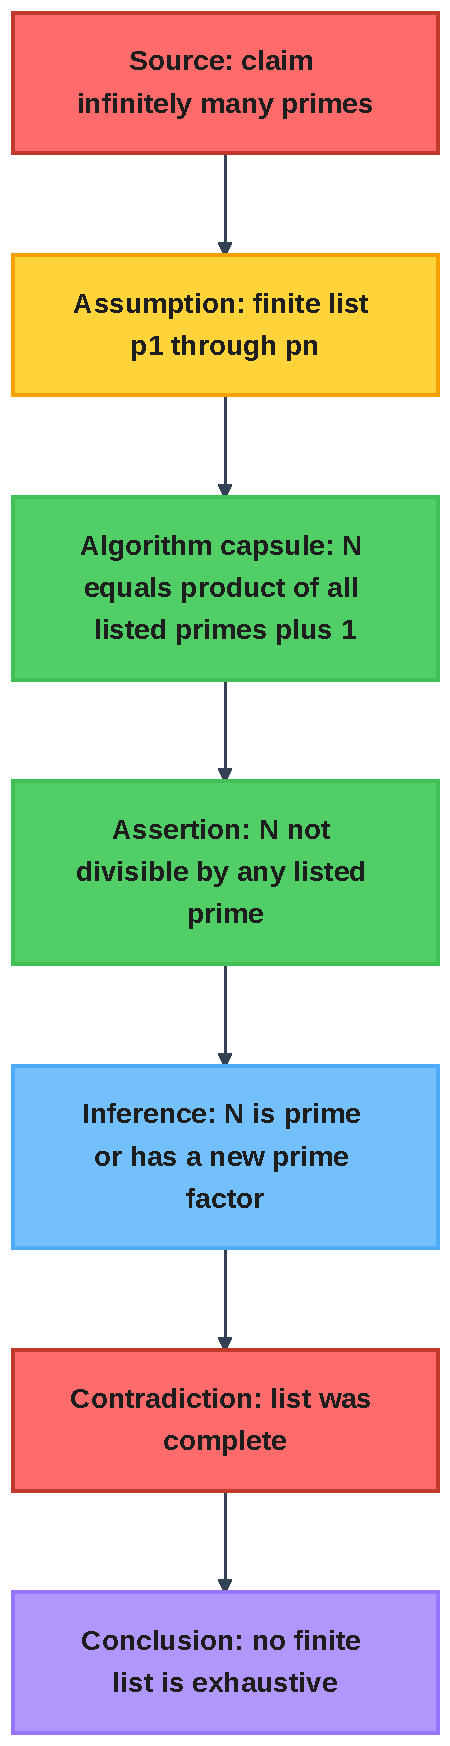
\includegraphics[width=\linewidth,height=0.78\textheight,keepaspectratio]{figures/fig3.pdf}
\end{minipage}\hfill
\noindent\begin{minipage}[t]{0.48\linewidth}
\centering
\textbf{Lean-schematic proof tree (goal and lemma oriented).}\\[0.6em]
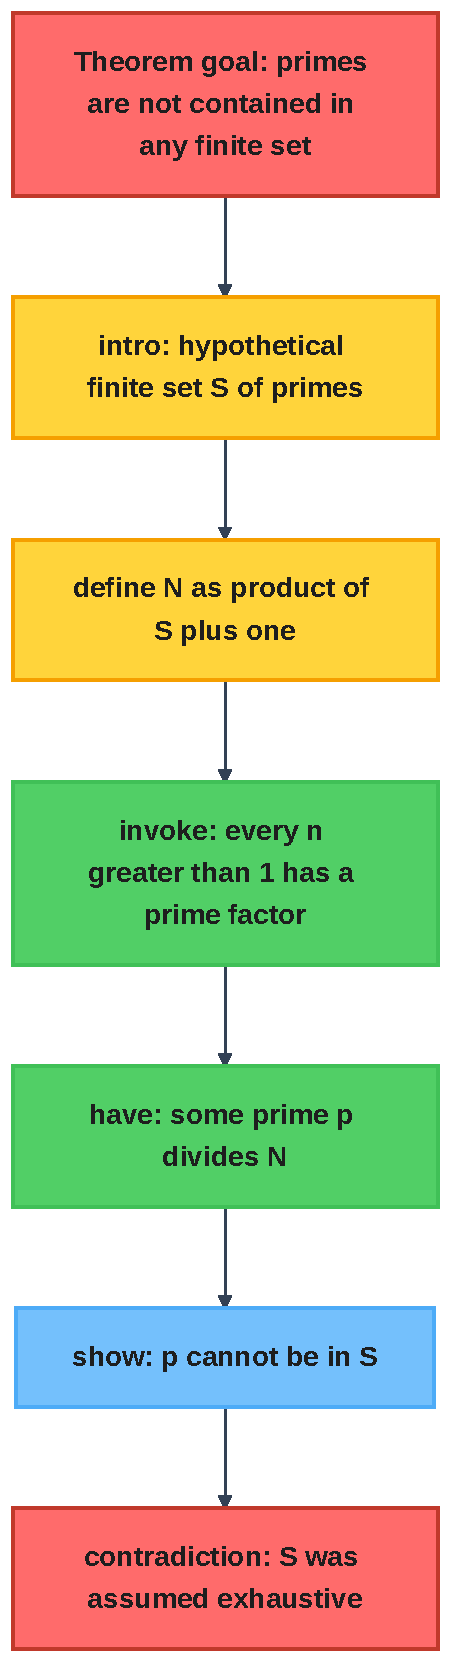
\includegraphics[width=\linewidth,height=0.78\textheight,keepaspectratio]{figures/fig4.pdf}
\end{minipage}

\textbf{How the two differ:}

\begin{longtable}[]{@{}>{\raggedright\arraybackslash}p{0.16\linewidth}>{\raggedright\arraybackslash}p{0.38\linewidth}>{\raggedright\arraybackslash}p{0.36\linewidth}@{}}
\toprule\noalign{}
Dimension & Informal proof graph (this paper) & Lean-style schematic \\
\midrule\noalign{}
\endhead
\bottomrule\noalign{}
\endlastfoot
\textbf{Node meaning} & Epistemic role (assumption, construction,
\ldots) & Goal state, definition, or lemma application \\
\textbf{Edges} & Justifies or explains for a human reader & Resolves
subgoal or depends on lemma in library \\
\textbf{Correctness} & Human review; not machine-checked &
Kernel-checkable when fully formalized \\
\textbf{Granularity} & Chosen for clarity; steps may be coarse & Often
fine-grained, many small tactic steps \\
\textbf{Construction} & LLM from prose, reviewed by author & Tactics or
proof terms \\
\textbf{Algorithm capsule} & Explicit node type for procedural content &
Corresponds to computable definitions inside terms \\
\end{longtable}

\textbf{Takeaway.} Lean proofs and informal proof graphs are
complementary: Lean answers "is this formally correct?"; proof graphs
answer "how is the argument organized for inspection, teaching, and
cross-proof comparison?" A natural research direction --- noted in §8
--- is to map or align Lean proof terms or tactic traces to role-labeled
graphs so the same theorem can be viewed in both registers. That
pipeline does not exist in the current Mathematics Database corpus,
which remains informal and LLM-derived.

\hypertarget{42-loops-back-edges-and-iterative-structure}{%
\subsubsection{4.2 Loops, Back-Edges, and Iterative
Structure}\label{42-loops-back-edges-and-iterative-structure}}

Algorithmic flowcharts may contain genuine cycles --- back-edges that
represent iteration or recursion. Proof graphs, as argued in §3.3, are
DAGs at the proof level but may contain cycles encapsulated within
algorithm capsule nodes.

One proof structure that appears to require a cycle at the proof level
is mathematical induction. In prose, induction "reapplies the same step"
at ever-larger indices, which suggests a loop. In the graph
representation, however, induction is better rendered as a back-edge
from the inductive step node to the inductive hypothesis node ---
semantically the same "next instance of the pattern," but a DAG with one
back-edge that displays reliably in Mermaid and preserves the
directional dependency structure.

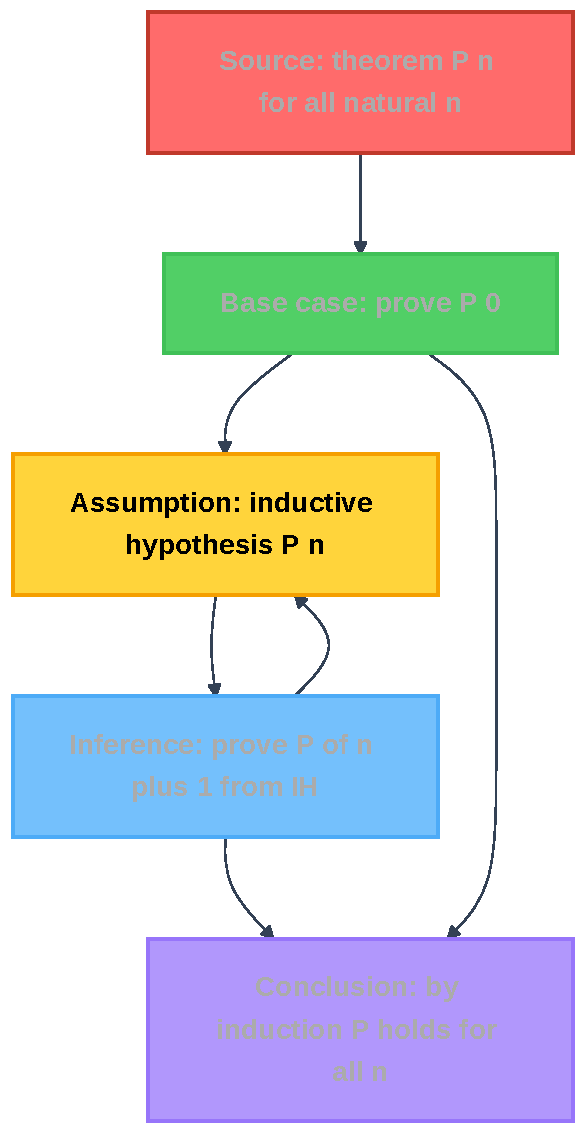
\includegraphics{figures/fig5.pdf}

The back-edge from ST to IH encodes the inductive pattern without
introducing a full cycle into the proof graph. This is a principled
representational choice: the back-edge marks where the inductive pattern
repeats without implying that the proof\textquotesingle s logical
dependency is circular.

This treatment of induction illustrates a general design principle for
proof graphs: \textbf{represent iterative proof patterns as back-edges
rather than self-loops}, both for Mermaid rendering reliability and for
logical clarity. Self-loops in Mermaid are rendered inconsistently
across versions; back-edges to a prior node are reliable and
semantically equivalent for the purposes of the proof graph
representation.

\hypertarget{43-merge-and-chain-topologies}{%
\subsubsection{4.3 Merge and Chain
Topologies}\label{43-merge-and-chain-topologies}}

Different proof strategies for the same theorem produce
characteristically different graph topologies. The Pythagorean Theorem
proof comparison entry in the Mathematics Database illustrates this most
clearly.

A geometric proof --- such as the similar-triangle construction --- fans
out into multiple construction nodes before converging on a central
algorithm capsule, producing a \textbf{merge topology}: width followed
by a join. An algebraic proof --- proceeding by symbolic rewriting ---
produces a \textbf{chain topology}: a narrow sequential path of
inference nodes with few constructions and shallow branching. The two
topologies are shown side by side below.

\noindent\begin{minipage}[t]{0.48\linewidth}
\centering
\textbf{Merge topology (geometric proof).}\\[0.6em]
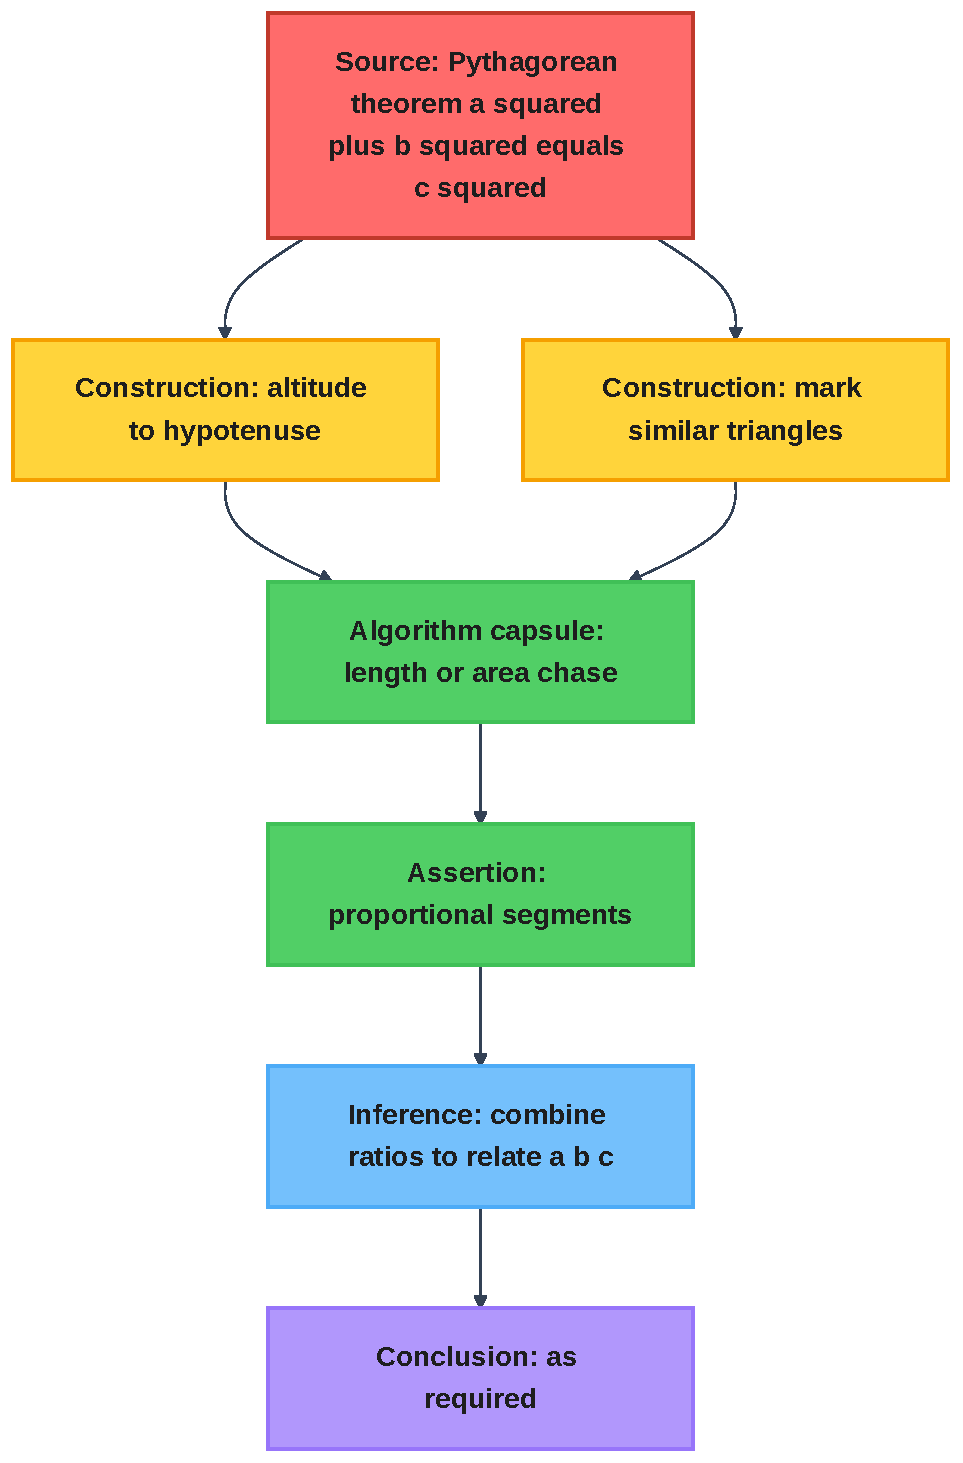
\includegraphics[width=\linewidth,height=0.78\textheight,keepaspectratio]{figures/fig6.pdf}
\end{minipage}\hfill
\noindent\begin{minipage}[t]{0.48\linewidth}
\centering
\textbf{Chain topology (algebraic proof).}\\[0.6em]
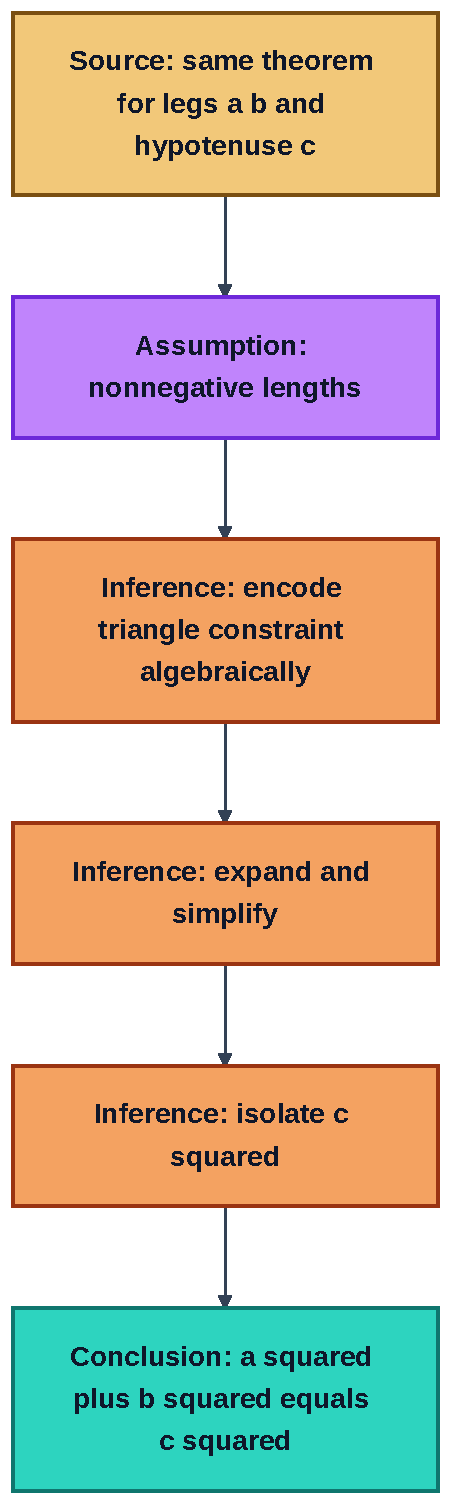
\includegraphics[width=\linewidth,height=0.78\textheight,keepaspectratio]{figures/fig7.pdf}
\end{minipage}

\begin{longtable}[]{@{}>{\raggedright\arraybackslash}p{0.16\linewidth}>{\raggedright\arraybackslash}p{0.38\linewidth}>{\raggedright\arraybackslash}p{0.36\linewidth}@{}}
\toprule\noalign{}
Topology & Visual signature & Typical role mix \\
\midrule\noalign{}
\endhead
\bottomrule\noalign{}
\endlastfoot
Merge (geometric) & Width then join into capsule & Several Construction
and Algorithm capsule nodes \\
Chain (algebraic) & Serial inferences, shallow branching & Predominantly
Inference, few constructions \\
Contradiction hub & Dense assumption/inference subgraph feeding single
contradiction node & High Assumption and Inference count, minimal
conclusion arc \\
Back-edge (induction) & Loop from inductive step to hypothesis & One
Assumption node, repeated inferential pattern \\
\end{longtable}

These topological signatures are visible by inspection and measurable by
the metadata fields in the Mathematics Database schema. They constitute
a vocabulary for describing what a proof graph looks like beyond raw
node counts --- and they are the basis for the cross-proof-family
comparisons developed in §6.3.

\hypertarget{44-conjunctive-premises-and-and-structure}{%
\subsubsection{4.4 Conjunctive Premises and AND
Structure}\label{44-conjunctive-premises-and-and-structure}}

A structural distinction important in proof graphs but not in
algorithmic flowcharts is the difference between \textbf{alternative
paths} and \textbf{joint premises}. In an algorithm, multiple edges
pointing to a single node typically mean that control may arrive from
alternative paths --- an OR structure. In a proof, multiple edges
pointing to a single node typically mean that all the incoming steps are
required together --- a conjunctive or AND structure representing joint
justification.

In the Mathematics Database as currently deployed, this distinction is
carried by node labels and colors rather than by distinct graph syntax.
A design iteration under evaluation introduces a compact hexagonal AND
marker for conjunctive joins, making joint justification explicitly
visible in the graph without requiring a large decorative node. The
working principle is to reserve AND markers for semantically important
conjunctions --- cases where the joint requirement of multiple premises
is itself a proof-theoretic observation worth marking --- rather than
applying them uniformly to every node with multiple predecessors.

This design question --- how to represent conjunctive premise structure
without visual noise --- is an open one for the proof graph
representation and is noted here as a known limitation and active
development direction.

\begin{center}\rule{0.5\linewidth}{0.5pt}\end{center}

\hypertarget{5-the-mathematics-database}{%
\subsection{5. The Mathematics
Database}\label{5-the-mathematics-database}}

The three graph types and their topological properties described in §3
and §4 are implemented in the Mathematics Database --- a publicly
accessible corpus of LLM-generated graphs stored as versioned JSON
metadata and rendered through an interactive HTML viewer.

\hypertarget{51-architecture}{%
\subsubsection{5.1 Architecture}\label{51-architecture}}

The Mathematics Database is implemented as a collection of JSON metadata
files stored on Google Cloud Storage, with an interactive HTML viewer
that renders the data in three sortable tables --- algorithms, axiomatic
theories, and proof graphs --- and generates live Mermaid diagram
previews.

Each entry in the database is a JSON object. The normative schema used
in this paper --- expressed in JSON Schema {[}15{]} --- is:

\begin{Shaded}
\begin{Highlighting}[]
\FunctionTok{\{}
  \DataTypeTok{"id"}\FunctionTok{:} \StringTok{"string"}\FunctionTok{,}
  \DataTypeTok{"title"}\FunctionTok{:} \StringTok{"string"}\FunctionTok{,}
  \DataTypeTok{"category"}\FunctionTok{:} \StringTok{"algorithm | axiomatic\_system | proof\_graph | hybrid"}\FunctionTok{,}
  \DataTypeTok{"subcategory"}\FunctionTok{:} \StringTok{"string"}\FunctionTok{,}
  \DataTypeTok{"graph\_type"}\FunctionTok{:} \StringTok{"flowchart | dependency | proof | hybrid"}\FunctionTok{,}
  \DataTypeTok{"complexity"}\FunctionTok{:} \StringTok{"low | medium | high"}\FunctionTok{,}
  \DataTypeTok{"nodes"}\FunctionTok{:} \ErrorTok{integer}\FunctionTok{,}
  \DataTypeTok{"edges"}\FunctionTok{:} \ErrorTok{integer}\FunctionTok{,}
  \DataTypeTok{"conditionals"}\FunctionTok{:} \ErrorTok{integer}\FunctionTok{,}
  \DataTypeTok{"and\_gates"}\FunctionTok{:} \ErrorTok{integer}\FunctionTok{,}
  \DataTypeTok{"or\_gates"}\FunctionTok{:} \ErrorTok{integer}\FunctionTok{,}
  \DataTypeTok{"not\_gates"}\FunctionTok{:} \ErrorTok{integer}\FunctionTok{,}
  \DataTypeTok{"loops"}\FunctionTok{:} \ErrorTok{integer}\FunctionTok{,}
  \DataTypeTok{"algorithm\_capsules"}\FunctionTok{:} \ErrorTok{integer}\FunctionTok{,}
  \DataTypeTok{"temporary\_assumptions"}\FunctionTok{:} \ErrorTok{integer}\FunctionTok{,}
  \DataTypeTok{"mermaid"}\FunctionTok{:} \StringTok{"string"}\FunctionTok{,}
  \DataTypeTok{"collections"}\FunctionTok{:} \OtherTok{[}\StringTok{"string"}\OtherTok{]}\FunctionTok{,}
  \DataTypeTok{"frontier"}\FunctionTok{:} \ErrorTok{boolean}\FunctionTok{,}
  \DataTypeTok{"source"}\FunctionTok{:} \StringTok{"string"}\FunctionTok{,}
  \DataTypeTok{"llm\_version"}\FunctionTok{:} \StringTok{"string"}\FunctionTok{,}
  \DataTypeTok{"version"}\FunctionTok{:} \StringTok{"string"}
\FunctionTok{\}}
\end{Highlighting}
\end{Shaded}

The deployed manifest uses \texttt{name} in place of \texttt{title} and
\texttt{processType} in place of \texttt{category} for implementation
compatibility. All other fields are identical between the normative
schema and the deployed manifest.

The analytical focus of this paper is the eight-entry \textbf{proof
graph corpus} documented in §5.3. The broader Mathematics Database ---
produced by the same pipeline --- also contains 23 algorithmic
flowcharts and 194 axiomatic dependency graphs (see §5.4 for the full
manifest). Those entries supply comparative context in §6.2 but are not
catalogued here.

The \texttt{frontier} flag marks entries where the graph representation
pushes against the limits of Mermaid\textquotesingle s expressivity or
the LLM\textquotesingle s reliability --- cases requiring additional
validation or suggesting future extensions to the methodology. One proof
graph entry currently carries this flag: the Kirby--Paris/Goodstein
Independence result, noted in §6.1.

\hypertarget{52-named-collections}{%
\subsubsection{5.2 Named Collections}\label{52-named-collections}}

The database includes named collections --- curatorial groupings of
entries by mathematician or theorem family. Their purpose is
navigational: a reader interested in Cantor\textquotesingle s work, or
Gödel\textquotesingle s foundational results, or
Euclid\textquotesingle s geometry can locate all relevant entries
together without searching by subcategory. Named collections currently
cover 63 mathematicians and 32 theorem families, for a total of 95
groupings. They are a discoverability feature rather than a formal
structural category and carry no analytical weight in the corpus
metrics.

\hypertarget{53-corpus-overview}{%
\subsubsection{5.3 Corpus Overview}\label{53-corpus-overview}}

Table 1 gives exact node, edge, and algorithm capsule counts for all
eight proof graph entries in the May 2026 manifest, drawn directly from
the deployed metadata.

\emph{Table 1: Proof graph corpus --- exact figures from May 2026
manifest.}

\begin{longtable}[]{@{}llllll@{}}
\toprule\noalign{}
Entry & Nodes & Edges & Capsules & Temp. Assumptions & Frontier \\
\midrule\noalign{}
\endhead
\bottomrule\noalign{}
\endlastfoot
Euclid Book I bundle & 41 & 48 & 1 & 0 & --- \\
Pythagorean Theorem & 33 & 39 & 2 & 0 & --- \\
Infinitely Many Primes & 14 & 17 & 1 & 1 & --- \\
Fundamental Theorem of Arithmetic & 27 & 34 & 2 & 1 & --- \\
Kirby--Paris / Goodstein & 10 & 9 & 1 & 0 & yes \\
Cantor Diagonal Proofs & 42 & 50 & 1 & 0 & --- \\
Gödel Completeness & 15 & 15 & 1 & 0 & --- \\
Gödel First Incompleteness & 14 & 13 & 1 & 0 & --- \\
\textbf{Totals} & \textbf{196} & \textbf{225} & \textbf{10} & \textbf{2}
& \\
\textbf{Averages} & \textbf{24.5} & \textbf{28.1} & \textbf{1.25} &
\textbf{0.25} & \\
\end{longtable}

All eight proof graph entries contain at least one algorithm capsule.
Within the Euclid Book I bundle, only proposition I.1 contributes a
capsule --- I.4 and I.5 carry individual construction nodes rather than
capsules --- as discussed in §6.1. The average of 24.5 nodes and 28.1
edges per proof graph is roughly double the typical algorithmic
flowchart in the same manifest, reflecting the higher inferential
overhead of justification relative to procedure.

\hypertarget{54-live-database}{%
\subsubsection{5.4 Live Database}\label{54-live-database}}

The Mathematics Database is publicly accessible at:

\url{https://storage.googleapis.com/regal-scholar-453620-r7-podcast-storage/mathematics-processes-database/mathematics-database-table.html}

Interactive viewers for all three graph types, including live Mermaid
rendering, are available at:

\url{https://huggingface.co/spaces/garywelz/programming_framework}

An experimental viewer demonstrating the compact hexagonal AND marker
grammar and revised proof-role palette --- discussed in §4.4 --- is
available for the Infinitely Many Primes proof graph at:

\url{https://storage.googleapis.com/regal-scholar-453620-r7-podcast-storage/mathematics-processes-database/proof-graphs/infinitely-many-primes-v2-demo.html}

This URL should be understood as a shape-and-palette demonstration. The
main corpus tables use the rectangular default rendering until migration
and validation are complete.

\begin{center}\rule{0.5\linewidth}{0.5pt}\end{center}

\hypertarget{6-findings-from-the-proof-graph-corpus}{%
\subsection{6. Findings from the Proof Graph
Corpus}\label{6-findings-from-the-proof-graph-corpus}}

This section reports three findings from the eight-entry proof graph
corpus (Table 1, §5.3): the diagonalization family spanning Cantor,
Gödel, and Goodstein (§6.1), structural complexity differences between
proof graphs and other graph types (§6.2), and topological differences
between proof families for the same theorem (§6.3).

\hypertarget{61-the-diagonalization-family}{%
\subsubsection{6.1 The Diagonalization
Family}\label{61-the-diagonalization-family}}

The central finding of this corpus study is that three landmark
diagonalization proofs --- Cantor\textquotesingle s diagonal arguments,
Gödel\textquotesingle s First Incompleteness Theorem, and the
Kirby--Paris/Goodstein independence result --- form a structurally
coherent \textbf{diagonalization family} when represented as proof
graphs. In each case an \textbf{algorithm capsule} is not incidental to
the proof but is its structural core --- the mechanism by which the
argument achieves its result.

In the Cantor diagonal proofs the capsule is the construction of a real
number, subset, or enumeration path that differs from every element of
an assumed listing --- a finite procedure applied at each position of an
infinite list. In the Gödel First Incompleteness proof graph the capsule
is the diagonal lemma: the arithmetical procedure that constructs a
self-referential sentence by applying a provability predicate to its own
Gödel number. In the Kirby--Paris/Goodstein entry the capsule is the
Goodstein sequence computation --- an explicit algorithmic procedure
whose termination, provable by ordinal descent, cannot be established
within Peano Arithmetic.

Figure 8 shows the family\textquotesingle s archetype as it appears in
the Cantor Diagonal Proofs database entry: the proof graph for the
uncountability of the reals in (0,1). The algorithm capsule --- read the
\emph{n}th digit of the \emph{n}th listed real and flip it --- sits at
the structural center of the graph. Everything upstream of the capsule
prepares its input (the assumed enumeration, written as decimal rows);
everything downstream is inference about its output (the anti-diagonal
real \emph{x}), terminating at the contradiction hub where the
completeness assumption collapses.

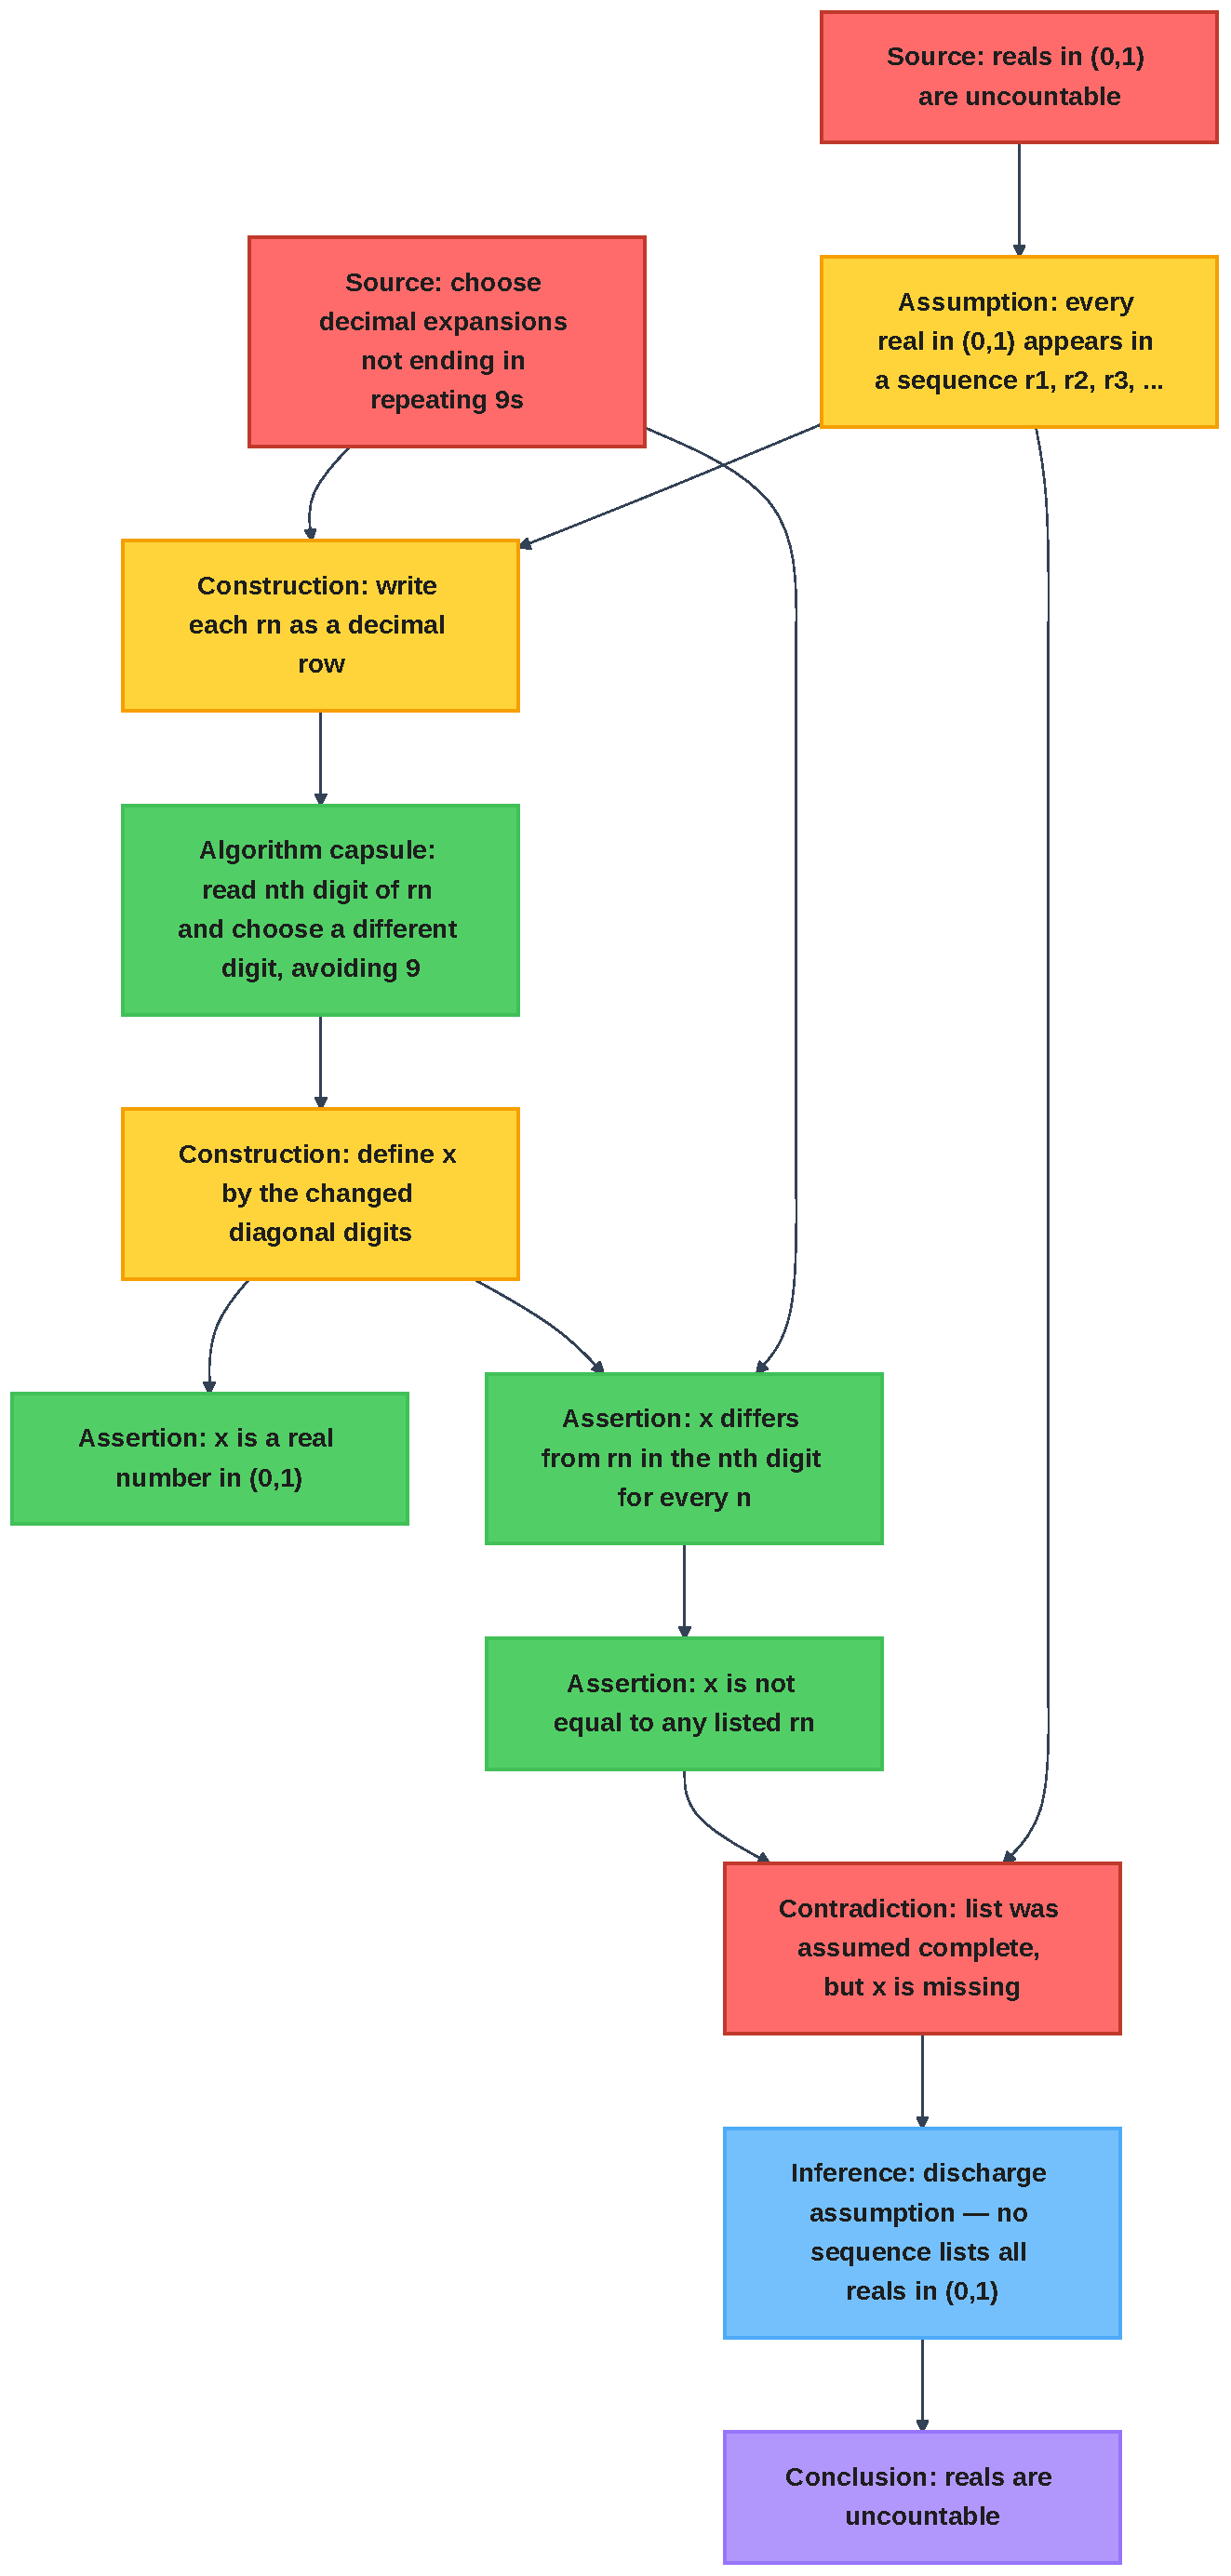
\includegraphics{figures/fig8.pdf}

\emph{Figure 8: Cantor\textquotesingle s diagonal argument for the
uncountability of the reals in (0,1), rendered as a proof graph (from
the Cantor Diagonal Proofs entry in the Mathematics Database). The
algorithm capsule (the anti-diagonal digit procedure) is the structural
core: assumptions and constructions feed it, assertions flow from it,
and the argument terminates at the contradiction hub. Colors follow the
GLMP 6-color role scheme: Red = source/contradiction, Yellow =
assumption/construction, Green = assertion/algorithm capsule, Light blue
= inference, Violet = conclusion.}

This is what diagonalization \emph{looks like} under the proof graph
representation, and the shape is visibly different from the other proof
shapes in the corpus. Two features mark the family at a glance. First,
the construction narrows to a waist at the algorithm capsule: everything
the proof builds funnels through the diagonal procedure before any
assertion can be made, in contrast to the chain topology of algebraic
proofs (§4.3), which has no procedural bottleneck at all. Second, the
assumption node throws a long edge that bypasses the entire construction
and lands directly on the contradiction node --- the visual trace of
self-reference, in which the assumed enumeration is confronted with an
object built from that very enumeration. Neither feature is apparent
from the prose of the proof; both are immediate in the picture. This is
the sense in which the representation itself is a finding: diagonal
proofs do not merely \emph{work} differently from other proofs --- under
this representation, they \emph{look} different.

All three capsules have the same logical role: they construct an object
with a property that generates the proof\textquotesingle s central
tension, whether contradiction, unprovability, or independence. The
proof graph representation makes this family resemblance visible and
measurable. All three entries share a common topological signature: a
dense algorithm capsule node with high out-degree feeding into an
assertion chain that terminates either at a contradiction node (Cantor,
Gödel) or a meta-level independence node (Kirby--Paris). This signature
is not accessible from prose descriptions of the three proofs, which
present them as belonging to different mathematical domains --- set
theory, mathematical logic, and combinatorics respectively.

The Gödel Numbering algorithm --- included in the corpus as a standalone
algorithmic flowchart --- serves as the explicit capsule twin to the
First Incompleteness proof graph, making this the first algorithm/proof
pair in the corpus where the same mathematical content appears in both
categories. This pairing directly supports the claim in §1.2: placing
proofs and algorithms in a common representational space reveals
structural relationships invisible when the two object types are
represented separately.

\textbf{Scope note.} Gödel\textquotesingle s second incompleteness
theorem is represented in the current database only as an axiomatic
dependency chart (Peano and Gödel sequence, Part 8). A dedicated proof
graph for second incompleteness is deferred: it requires additional
internal formalization of consistency statements and would exceed the
validation burden of the first incompleteness pilot.

Beyond the diagonalization family, algorithm capsules appear in all
eight proof graph entries (Table 1). What the proof graph representation
makes explicit --- and measurable --- is the structural boundary between
the algorithmic and the inferential within a single proof. That boundary
is visible in the graph and absent from prose.

Within the Euclid Book I bundle, the fact that only proposition I.1
contributes a capsule is instructive. I.4 (SAS Congruence) has zero
capsules because its proof proceeds entirely by superposition: a
methodological assumption rather than a construction. I.5 (Base Angles)
has zero capsules because its construction steps are individual
proof-specific auxiliary lines rather than a reusable procedure. The
contrast between I.1, I.4, and I.5 within the same bundle illustrates
the decision rule stated in §3.3: a capsule is a self-contained
procedural substructure with its own input/output logic, not merely a
sequence of construction steps.

\hypertarget{62-structural-complexity-comparison}{%
\subsubsection{6.2 Structural Complexity
Comparison}\label{62-structural-complexity-comparison}}

The database\textquotesingle s quantitative metadata enables direct
complexity comparison across mathematical objects that are not usually
compared. Using the exact figures from Table 1, the eight proof graph
entries average 24.5 nodes and 28.1 edges --- roughly double the typical
algorithmic flowchart in the same manifest. Individual proof graphs
range from 10 nodes and 9 edges (Kirby--Paris/Goodstein, frontier) to 42
nodes and 50 edges (Cantor Diagonal Proofs bundle).

Three structural observations follow from the corpus metadata:

\textbf{Proof graphs are more complex than algorithmic flowcharts of
comparable mathematical content.} The higher node and edge counts
reflect the inferential overhead of justification relative to procedure:
a proof must not only perform a computation but establish why the
computation\textquotesingle s output has the required property. The
algorithm capsule node type makes this overhead visible by marking where
procedure ends and inference begins.

\textbf{Proof graphs differ in complexity from axiomatic dependency
graphs of related content.} Axiomatic charts in the broader database
(e.g., Peano Arithmetic, ZFC) vary in depth-to-breadth ratio; proof
graphs for the same domain allocate complexity differently, with higher
inferential overhead reflected in node and edge counts.

\textbf{Proof-by-contradiction graphs have a distinctive topology.} A
single contradiction node with high in-degree, preceded by a dense
assumption and inference subgraph, followed by a minimal conclusion arc.
This contradiction hub topology is visible in the Cantor, Gödel, and
Infinitely Many Primes entries and is one of the topological signatures
identified in §4.3.

These observations are grounded in exact figures from a small,
manifest-documented corpus of eight proof graphs. They should be
understood as findings from a systematic pilot rather than large-scale
statistical claims. A larger corpus --- developed through the community
extension process described in §8 --- would support stronger statistical
inference.

\hypertarget{63-cross-proof-family-comparison}{%
\subsubsection{6.3 Cross-Proof-Family
Comparison}\label{63-cross-proof-family-comparison}}

The Pythagorean Theorem proof comparison entry demonstrates a capability
unique to the graph-theoretic approach: direct structural comparison of
multiple proofs of the same theorem. The entry captures several distinct
proof families --- geometric, algebraic, and trigonometric --- in a
single hybrid graph, with node colors encoding proof family membership.

The topological contrast between proof families, developed in §4.3,
becomes metrically grounded here. Geometric proofs allocate complexity
differently from algebraic proofs: more construction nodes and algorithm
capsules in the geometric family, longer inference chains and fewer
constructions in the algebraic family, more assumption nodes in the
trigonometric family (which requires more lemmas about trigonometric
identities as starting points).

These differences are difficult to articulate precisely in prose. In the
graph representation they are visible by inspection and measurable from
the metadata. A proof with two construction nodes and two capsules
feeding a single algorithm capsule hub has a different structural
character from a proof with five sequential inference nodes and no
capsules --- and that difference is now expressible as a metric rather
than a qualitative judgment.

The Pythagorean Theorem entry is the proof graph
corpus\textquotesingle s clearest demonstration that the representation
enables a new kind of mathematical comparison: not "which proof is more
elegant" --- a judgment that depends on aesthetic criteria --- but
"which proof allocates its structural complexity differently, and in
what specific ways." That is a question the graph representation can
answer precisely.

\begin{center}\rule{0.5\linewidth}{0.5pt}\end{center}

\hypertarget{7-limitations}{%
\subsection{7. Limitations}\label{7-limitations}}

\textbf{LLM accuracy.} LLM-generated proof graphs may misrepresent the
logical structure of proofs, particularly for complex or non-standard
arguments. All entries in the current database have been reviewed by the
author, but systematic expert validation --- particularly by logicians
and proof theorists --- remains future work. The human-in-the-loop
pipeline described in §2.3 mitigates but does not eliminate this risk.

\textbf{Mermaid expressivity.} Mermaid does not natively support some
features that would be useful for proof graphs: parallel proof branches,
multiple inheritance in axiomatic hierarchies, or quantifier structure.
The most consequential expressivity limitation is the representation of
conjunctive premises --- distinguishing joint justification from
alternative control flow paths. The AND marker grammar described in §4.4
addresses this partially; it remains under evaluation and has not yet
been rolled out across the main corpus. These limitations are otherwise
managed by approximation and noted in individual entry metadata.

\textbf{The DAG assumption and encapsulated cycles.} Proof graphs in
this corpus are treated as DAGs at the proof level, with cycles
encapsulated within algorithm capsule nodes. This is a principled
representational choice, as argued in §3.3, but it means that the
internal structure of capsule nodes is not fully represented in the
top-level graph. A proof graph representation that exposed
capsule-internal structure as a subgraph would be more expressive but
significantly more complex to generate, validate, and render. This is a
known limitation of the current implementation.

\textbf{Corpus size.} The proof graph corpus contains eight entries
across five mathematical domains. The findings in §6 are grounded in
exact figures from this corpus but should be understood as findings from
a systematic pilot rather than large-scale statistical claims. The
observations about the diagonalization family, contradiction hub
topology, and cross-proof-family complexity differences are structurally
well-motivated but would benefit from a larger corpus for statistical
confirmation.

\textbf{No formal semantics.} The graph representations are visually and
structurally informative but do not carry formal logical semantics. They
are not machine-verifiable in the sense of proof assistants. They are
human-readable and machine-processable structural descriptions --- a
complement to formal verification systems rather than a substitute for
them. The relationship to formal proof assistants is discussed in §4.1.

\textbf{Single author, single pipeline.} All current entries were
generated and reviewed by a single author using a single LLM pipeline.
Inter-rater reliability and multi-pipeline reproducibility have not been
evaluated. This is a standard limitation of first-generation corpus
construction and is noted here for transparency.

\begin{center}\rule{0.5\linewidth}{0.5pt}\end{center}

\hypertarget{8-future-directions}{%
\subsection{8. Future Directions}\label{8-future-directions}}

\textbf{Capsule-internal structure as subgraphs.} The current
implementation encapsulates cyclic and iterative structures within
algorithm capsule nodes, preserving DAG structure at the proof level. A
natural extension is to expose capsule-internal structure as explicit
subgraphs --- rendering the diagonal enumeration in the Cantor proofs or
the Goodstein sequence computation in the Kirby--Paris entry as fully
expanded flowcharts linked to their parent proof graphs. This would make
the two-level DAG/cycle structure described in §3.3 and §7 fully visible
and navigable rather than implied by the capsule node type. The
technical challenge is rendering complexity: subgraph expansion would
significantly increase diagram size and may require a viewer interface
that supports expand/collapse navigation rather than static Mermaid
rendering.

\textbf{Integration with proof assistants.} The Lean 4 mathematical
library (Mathlib) and the Coq Proof Assistant contain large bodies of
formalized mathematics. As sketched in §4.1, informal proof graphs and
Lean-style proof structures are complementary rather than competing
representations: Lean answers "is this formally correct?" while proof
graphs answer "how is the argument organized for inspection and
comparison?" A natural research direction is to align the two --- mining
tactic traces or proof terms from Lean into role-labeled graphs, or
using Mathlib entries as ground truth for validating corpus entries.
This pipeline does not exist in the current database but would
significantly increase both corpus size and validation quality.

\textbf{Systematic corpus validation and metadata quality.} The manifest
correction identified during preparation of this paper --- the Euclid
Book I bundle capsule count requiring update from 0 to 1 --- points to a
broader need for systematic metadata validation across the corpus. A
validation pipeline that checks field consistency, flags zero-capsule
proof graph entries for review, and cross-checks node and edge counts
against rendered diagrams would improve corpus quality and
reproducibility. This is particularly important before community
extension, where submitted entries will not have been generated by the
same author using the same pipeline.

\textbf{Community extension.} A community-driven submission and review
process, modeled on arXiv or Zenodo, would enable other researchers to
contribute entries, validate existing ones, and propose new named
collections. The Mathematics Database\textquotesingle s current
single-author, single-pipeline construction is appropriate for a pilot
corpus but limits scale and reproducibility. Community extension would
require the validation pipeline described above as a prerequisite.

\textbf{Cross-domain comparison across the Programming Framework.} The
Programming Framework has been applied across biology, chemistry,
physics, computer science, and mathematics. The most ambitious extension
of the present work is systematic comparison across the
discipline-specific databases --- identifying structural regularities
that appear across domains and asking whether the algorithm capsule
concept, the contradiction hub topology, or the DAG/cycle two-level
structure have analogs in non-mathematical process graphs. This is the
subject of a planned comparative paper.

\textbf{AI-assisted mathematics education.} The Mathematics
Database\textquotesingle s interactive viewers suggest a natural
application in mathematics education. Students can explore the
dependency structure of theorems, trace proof paths from axioms, and
compare the structural complexity of different proofs of the same
result. The named collections --- grouping entries by mathematician or
theorem family --- provide entry points organized around the historical
narrative of mathematics rather than formal subcategory. Development of
educational interfaces tailored to undergraduate and graduate
mathematics curricula is planned.

\textbf{Proof-graph shape grammar.} The topological signatures
identified in §4.3 --- contradiction hub, merge, chain, back-edge ---
constitute the beginning of a shape grammar for proof graphs. Extending
this grammar systematically across the full corpus, testing whether the
signatures scale to more complex proofs such as the Cantor diagonal
family or the Fundamental Theorem of Arithmetic, and developing a formal
vocabulary for describing proof graph topology beyond raw node counts is
a natural next step. The AND marker grammar described in §4.4 is one
component of this; a complementary OR/case-split marker for genuine
alternative proof branches is a natural addition, to be used with the
same discipline of reserving markers for semantically important
structural features.

\begin{center}\rule{0.5\linewidth}{0.5pt}\end{center}

\hypertarget{9-conclusion}{%
\subsection{9. Conclusion}\label{9-conclusion}}

This paper has introduced proof graphs with algorithm capsules as a
diagrammatic representation of mathematical justification structure, and
reported a corpus study of eight proof graphs with a central finding:
three landmark diagonalization proofs --- Cantor, Gödel, and Goodstein
--- form a structurally coherent family whose common topological
signature is only visible in the graph representation. In each case the
algorithm capsule is not incidental to the proof but is its structural
core. This family resemblance cuts across the conventional domain
boundaries of set theory, mathematical logic, and combinatorics. It is a
finding about mathematical structure, not merely about representation.

All eight proof graph entries in the corpus contain at least one
algorithm capsule; the diagonalization family is the most structurally
pronounced instance of a broader regularity.

A skeptic might ask whether the graph representation merely redescribes
what a careful reader of the prose already knows. The answer developed
in §1.2 bears restating here: making structure explicit is itself a form
of discovery when the structure was previously inaccessible to
measurement and comparison. The diagonalization family is not visible in
prose descriptions of the three proofs. It becomes visible --- and
measurable, and comparable --- only when the three proofs are placed in
a common representational space. The same is true of the two-level
DAG/cycle structure identified in §3.3: proof graphs are acyclic at the
proof level but may contain cycles encapsulated within algorithm capsule
nodes. That structural property is present in the proofs whether or not
it is represented. The graph makes it nameable, inspectable, and
available for cross-proof comparison in a way that prose does not.

The proof graph node vocabulary --- eight roles encoding the
proof-theoretic function of each step --- and the algorithm capsule
concept are contributions to the general Programming Framework
vocabulary with applications beyond mathematics. Wherever embedded
procedural substructures appear within larger logical or justificatory
structures, the algorithm capsule node type provides a representational
handle that makes those substructures visible, nameable, and comparable.

The Mathematics Database is offered as open infrastructure: a starting
point that others can validate, extend, and critique. Its current scale
--- eight proof graphs, 194 axiomatic dependency graphs, 23 algorithmic
flowcharts --- is appropriate for a pilot corpus. The findings it
supports are structurally well-motivated and grounded in exact public
figures. A larger corpus, developed through the community extension and
validation processes described in §8, would support stronger claims.

The broader argument of this paper is that formal structure is
recoverable from natural language descriptions of complex systems, and
is meaningful, measurable, and comparable once recovered. That argument
was first made for procedural processes. This paper extends it to
logical dependency structures and justificatory structures. The same
representational move that makes algorithms inspectable as typed
computational graphs makes mathematical proofs inspectable as typed
justification graphs --- and in doing so reveals that some of the most
important proofs in the history of mathematics share a structural core
that their surface differences in domain and technique have long
obscured.

\begin{center}\rule{0.5\linewidth}{0.5pt}\end{center}

\hypertarget{references}{%
\subsection{References}\label{references}}

{[}1{]} G. Welz, \emph{The Programming Framework: A General Method for
Process Analysis Using LLMs and Mermaid Visualization}, Zenodo preprint,
DOI: 10.5281/zenodo.18463441, 2026.

{[}2{]} "The QED manifesto," in \emph{Automated Deduction --- CADE-12},
LNCS 814, Springer, 1994, pp. 237--251.

{[}3{]} J. Avigad, L. de Moura, S. Koon, and S. Ullrich, \emph{Theorem
Proving in Lean 4}, online textbook, Lean Community,
\url{https://lean-lang.org/theorem_proving_in_lean4/} (accessed May
2026).

{[}4{]} The mathlib Community, "The Lean mathematical library," in
\emph{Certified Programs and Proofs (CPP \textquotesingle20)}, ACM,
2020, pp. 130--144. DOI: 10.1145/3372885.3373824

{[}5{]} The Coq Development Team, \emph{The Coq Proof Assistant} ---
documentation and releases, \url{https://coq.inria.fr/} (accessed May
2026).

{[}6{]} T. Nipkow, L. C. Paulson, and M. Wenzel, \emph{Isabelle/HOL: A
Proof Assistant for Higher-Order Logic}, LNCS 2283, Springer, 2002.

{[}7{]} A. Grabowski, A. Korniłowicz, and A. Naumowicz, "Four decades of
Mizar," \emph{Journal of Automated Reasoning}, vol. 55, no. 3, pp.
191--198, 2015.

{[}8{]} OpenMath Society, \emph{The OpenMath Standard} (2.0 / ongoing
revisions), \url{https://www.openmath.org/} (accessed May 2026).

{[}9{]} J. Krajíček, \emph{Bounded Arithmetic, Propositional Logic, and
Complexity Theory}, Cambridge University Press, 1995.

{[}10{]} C. R. Twardy, "Argument maps improve critical thinking,"
\emph{Teaching Philosophy}, vol. 27, no. 1, pp. 1--22, 2004.

{[}11{]} OpenAI, "GPT-4 technical report," \emph{arXiv:2303.08774},
2024.

{[}12{]} A. Lewkowycz et al., "Solving quantitative reasoning problems
with language models," \emph{Nature}, vol. 619, pp. 471--478, 2022.

{[}13{]} S. Polu and I. Sutskever, "Generative language modeling for
automated theorem proving," \emph{arXiv:2009.03393}, 2020.

{[}14{]} K. Sveidqvist and contributors, \emph{Mermaid} --- diagram
syntax and toolkit, \url{https://www.mermaidjs.org/} (accessed May
2026).

{[}15{]} JSON Schema Consortium, \emph{JSON Schema: A Media Type for
Describing JSON Documents}, Draft 2020-12 and specifications,
\url{https://json-schema.org/} (accessed May 2026).

\begin{center}\rule{0.5\linewidth}{0.5pt}\end{center}

\hypertarget{acknowledgments}{%
\subsection{Acknowledgments}\label{acknowledgments}}

This work is part of the CopernicusAI Knowledge Engine project, which
aims to create AI-powered tools for scientific research synthesis and
knowledge discovery. The Mathematics Database and the Programming
Framework serve as foundational methodological components of that
project. The author thanks the CUNY Graduate Center New Media Lab for
institutional support.

The diagrams in this paper were generated with large-language-model
assistance as part of the Programming Framework methodology described
herein; large-language-model tools were also used to assist with
copy-editing and revision. All scholarly content, analysis, and
conclusions are the author\textquotesingle s own.

\end{document}
